\documentclass{report}
\usepackage[french]{babel} 
\usepackage[utopia]{mathdesign}

% Pour emojis et autres symbols de Extansive LaTeX symbols list 

% Permet d'ajuster la taille des marges et de la distance pour les footer
\usepackage[tmargin=2cm,rmargin=0.4in,lmargin=0.4in,bmargin=2cm,footskip=.2in]{geometry}

% Permet d'optimiser l'affichage de différents symboles et formules mathématiques
\usepackage{amsmath,amsthm,mathtools}
\usepackage[clock]{ifsym}
\usepackage{karnaugh-map}

\usepackage{svg}
% Modifie l'apparence des nombre en mathmode et textmode
%\usepackage[varbb]{newpxmath}

% Modifier l'apparence des fractions
\usepackage{xfrac}

            %%%%%%%%%%%%%%%%%  Sect.        14 Oct 2024     %%%%%%%%%%%%%%%%%%%%%%%%%%%%%%%%%%%%%%%%%%%%%%%%%%%%%%%%%%%
\usepackage{graphicx}
\usepackage{caption}
\usepackage{subcaption}
\usepackage{arydshln}
            %%%%%%%%%%%%%%%%%  Sect.        14 Oct 2024     %%%%%%%%%%%%%%%%%%%%%%%%%%%%%%%%%%%%%%%%%%%%%%%%%%%%%%%%%%%
\usepackage{balance}
\usepackage{dirtree}
\usepackage{titlesec}



% Chapters and sections
\usepackage{helvet}
\titleformat{\chapter}
  {\fontfamily{phv}\bfseries\huge} % format
  {}                % label
  {0pt}             % sep
  {\color{myb}\huge}           % before-code



\titleformat{\section}
  {\normalfont\scshape}{\thesection}{1em}{}
\usepackage{circuitikz}


% Customizing the spacing for the chapter titles
\titlespacing*{\chapter}{0pt}{0pt}{20pt}

% Allow hfill in math environment
\newcommand{\specialcell}[1]{\ifmeasuring@#1\else\omit$\displaystyle#1$\ignorespaces\fi}

% Allow you to do the non implication (implication barred)
\newcommand{\notimplies}{%
  \mathrel{{\ooalign{\hidewidth$\not\phantom{=}$\hidewidth\cr$\implies$}}}}



\DeclareRobustCommand{\looongrightarrow}{%
  \DOTSB\relbar\joinrel\relbar\joinrel\relbar\joinrel\rightarrow
}






% Permet de rayer (barrer) l'argument avec la touche
% \cancel{} \bcancel{} ou \xcancel{}
\usepackage[makeroom]{cancel}

% Extension du package amsmath; corrige certains bugs et déficiences de son prédecesseur
\usepackage{mathtools}

% This package provides most of the flexibility you may want to customize the three basic list
% environments (enumerate, itemize and description)
\usepackage{bookmark} 

% Réorganiser les théorèmes et Lemmes. Usage complexe. 
% Référence : https://ctan.math.illinois.edu/macros/latex/contrib/theoremref/theoremref-doc.pdf
\hypersetup{hidelinks}
\usepackage{hyperref,theoremref} 

% Fournit un environnement pour créer des boîtes colorées
\usepackage[most,many,breakable]{tcolorbox}


%\newcommand\mycommfont[1]{\footnotesize\ttfamily\textcolor{blue}{#1}}\SetCommentSty{mycommfont}

%\newcommand{\incfig}[1]{%\def\svgwidth{\columnwidth}\import{./figures/}{#1.pdf_tex}}
\newcommand{\arc}[1]{\wideparen{#1}}

%Pour colorer les lignes séparatrices de tableaux
\usepackage{colortbl}
\usepackage{tikzsymbols}

\usepackage{framed}
\usepackage{titletoc}
\usepackage{etoolbox}
\usepackage{lmodern}
\usepackage{tabularx}
\usepackage{enumitem}
\usepackage{amsthm}
            %%%%%%%%%%%%%%%%%  Sect.        14 Oct 2024     %%%%%%%%%%%%%%%%%%%%%%%%%%%%%%%%%%%%%%%%%%%%%%%%%%%%%%%%%%%

\usepackage{lipsum}
\usepackage{titling}
\renewcommand\maketitlehooka{\null\mbox{}\vfill}
\renewcommand\maketitlehookd{\vfill\null}

\newcommand{\varitem}[3][black]{%
  \item[%
   \colorbox{#2}{\textcolor{#1}{\makebox(5.5,7){#3}}}%
  ]
}
\usepackage{afterpage}
\newcommand\myemptypage{
    \null
    \thispagestyle{empty}
    \addtocounter{page}{-1}
    \newpage
    }


%=================== 
% Comand for target symbol 

\newcommand{\target}{%
  \begin{tikzpicture}[scale=0.5]
    \fill[black] (0,0) circle (0.1);
    \draw (0,0) circle (0.2);
    \draw (0,0) circle (0.3);
  \end{tikzpicture}%
}





% from https://tex.stackexchange.com/a/167024/121799
\newcommand{\ClaudioList}{red,DarkOrange1,Goldenrod1,Green3,blue!50!cyan,DarkOrchid2}
\newcommand{\SebastianoItem}[1]{\foreach \X[count=\Y] in \ClaudioList
{\ifnum\Y=#1\relax
\xdef\SebastianoColor{\X}
\fi
}
\tikz[baseline=(SebastianoItem.base),remember
picture]{%
\node[fill=\SebastianoColor,inner sep=4pt,font=\sffamily,fill opacity=0.5] (SebastianoItem){#1)};}
}
\newcommand{\SebastianoHighlight}{\tikz[overlay,remember picture]{%
\fill[\SebastianoColor,fill opacity=0.5] ([yshift=4pt,xshift=-\pgflinewidth]SebastianoItem.east) -- ++(4pt,-4pt)
-- ++(-4pt,-4pt) -- cycle;
}}   
            %%%%%%%%%%%%%%%%%  Sect.        14 Oct 2024     %%%%%%%%%%%%%%%%%%%%%%%%%%%%%%%%%%%%%%%%%%%%%%%%%%%%%%%%%%%





%====================================================================

%====================================================================
\newcommand*{\authorimg}[1]%
    { \raisebox{-1\baselineskip}{\includegraphics[width=\imagesize]{#1}}}
\newlength\imagesize  

\usepackage{pgfplots}
\pgfplotsset{compat=1.17}

%==========================================================================================
\usepackage{libris} 
\usepackage{etoolbox}
\usepackage[export]{adjustbox}% for positioning figures

\makeatletter
% Force le chapitre suivant sur la ligne succedant la fin du 
% chapitre précédent
\patchcmd{\chapter}{\if@openright\cleardoublepage\else\clearpage\fi}{}{}{}
\makeatother
\usepackage[Sonny]{fncychap}


%boîte de couleur grise
\tcbset{
  graybox/.style={
    colback=gray!20,
    colframe=black,
    sharp corners=downhill,
    boxrule=1pt,
    left=5pt,
    right=5pt,
    top=5pt,
    bottom=5pt,
    boxsep=0pt,
	 % <-- add four values for each corner
  }
}
\newtcolorbox{graybox}{graybox}

%==========================================================================================



\usepackage{xcolor}
\usepackage{varwidth}
\usepackage{varwidth}
\usepackage{etoolbox}
%\usepackage{authblk}
\usepackage{nameref}
\usepackage{multicol,array}
\usepackage{tikz-cd}
\usepackage[ruled,linesnumbered,ruled]{algorithm2e}
\usepackage{comment} % enables the use of multi-line comments (\ifx \fi) 
\usepackage{import}
\usepackage{xifthen}
\usepackage{pdfpages}
\usepackage{transparent}


%\usepackage[french]{babel}
\usepackage{listings} % pour écrire du code dans un environnement
\lstset{
  basicstyle=\ttfamily,
  columns=fullflexible,
  keepspaces=true
}
\usepackage{caption}
\usepackage{float} % Pour forcer les images au bon endroit



\usepackage[T1]{fontenc}
\usepackage{csquotes}
%%%%%%%%%%%%%%%%%%%%%%%%%%%%%%%%%%%%%%%%%%%%%%%%%%%%%%%%%%%%%%%%%%%%%%%%%%%%%%%%%%%%%%%%%%%%%%%%%
%									ENSEMBLE DE COULEURS
%%%%%%%%%%%%%%%%%%%%%%%%%%%%%%%%%%%%%%%%%%%%%%%%%%%%%%%%%%%%%%%%%%%%%%%%%%%%%%%%%%%%%%%%%%%%%%%%%

\definecolor{myg}{RGB}{56, 140, 70}
\definecolor{myb}{RGB}{45, 111, 177}

\definecolor{mygbg}{RGB}{235, 253, 241}


\definecolor{myr}{RGB}{199, 68, 64}
\definecolor{mytheorembg}{HTML}{F2F2F9}
\definecolor{mytheoremfr}{HTML}{00007B}
\definecolor{mylenmabg}{HTML}{FFFAF8}
\definecolor{mylenmafr}{HTML}{983b0f}
\definecolor{mypropbg}{HTML}{f2fbfc}
\definecolor{mypropfr}{HTML}{191971}
\definecolor{myexamplebg}{HTML}{F2FBF8}
\definecolor{myexamplefr}{HTML}{88D6D1}
\definecolor{myexampleti}{HTML}{2A7F7F}
\definecolor{mydefinitbg}{HTML}{E5E5FF}
\definecolor{mydefinitfr}{HTML}{3F3FA3}
\definecolor{notesgreen}{RGB}{0,162,0}
\definecolor{myp}{RGB}{197, 92, 212}
\definecolor{mygr}{HTML}{2C3338}
\definecolor{myred}{RGB}{127,0,0}
\definecolor{myyellow}{RGB}{169,121,69}
\definecolor{myexercisebg}{HTML}{F2FBF8}
\definecolor{myexercisefg}{HTML}{88D6D1}
\definecolor{myred}{RGB}{127,0,0}
\definecolor{myyellow}{RGB}{169,121,69}
\definecolor{LightLavender}{HTML}{DFC5FE}

\definecolor{blue}{HTML}{008ED7}
\definecolor{mygray}{gray}{0.75}
\definecolor{lightBlue}{RGB}{235, 245, 255}
\definecolor{tcbcolred}{RGB}{255,0,0}
\definecolor{myGreen}{HTML}{009900}

% command to circle a text
\newtcbox{\entoure}[1][red]{on line,
	arc=3pt,colback=#1!10!white,colframe=#1!50!black,
	before upper={\rule[-3pt]{0pt}{10pt}},boxrule=1pt,
	boxsep=0pt,left=2pt,right=2pt,top=1pt,bottom=.5pt}
% command for the circle for the number of part entries
\newcommand\Circle[1]{\tikz[overlay,remember picture]
	\node[draw,circle, text width=18pt,line width=1pt] {#1};}

\newtcbox{\entouree}[1][red]{on line,
	arc=3pt,colback=#1!10!white,colframe=#1!50!white,
	before upper={\rule[-3pt]{0pt}{10pt}},boxrule=1pt,
	boxsep=0pt,left=2pt,right=2pt,top=1pt,bottom=.5pt}

\newcommand{\shellcmd}[1]{\\\indent\indent\texttt{\footnotesize\# #1}\\}

%=====================================================================

\patchcmd{\tableofcontents}{\contentsname}{\rmfamily\contentsname}{}{}
% patching of \@part to typeset the part number inside a framed box in its own line
% and to add color
\makeatletter
\patchcmd{\@part}
  {\addcontentsline{toc}{part}{\thepart\hspace{1em}#1}}
  {\addtocontents{toc}{\protect\addvspace{20pt}}
    \addcontentsline{toc}{part}{\huge{\protect\color{myyellow}%
      \setlength\fboxrule{2pt}\protect\Circle{%
        \hfil\thepart\hfil%
      }%
    }\\[2ex]\color{myred}\rmfamily#1}}{}{}

%\patchcmd{\@part}
%  {\addcontentsline{toc}{part}{\thepart\hspace{1em}#1}}
%  {\addtocontents{toc}{\protect\addvspace{20pt}}
%    \addcontentsline{toc}{part}{\huge{\protect\color{myyellow}%
%      \setlength\fboxrule{2pt}\protect\fbox{\protect\parbox[c][1em][c]{1.5em}{%
%        \hfil\thepart\hfil%
%      }}%
%    }\\[2ex]\color{myred}\sffamily#1}}{}{}
\makeatother
% this is the environment used to typeset the chapter entries in the ToC
% it is a modification of the leftbar environment of the framed package
\renewenvironment{leftbar}
  {\def\FrameCommand{\hspace{6em}%
    {\color{myyellow}\vrule width 2pt depth 6pt}\hspace{1em}}%
    \MakeFramed{\parshape 1 0cm \dimexpr\textwidth-6em\relax\FrameRestore}\vskip2pt%
  }
 {\endMakeFramed}

% using titletoc we redefine the ToC entries for parts, chapters, sections, and subsections
\titlecontents{part}
  [0em]{\centering}
  {\contentslabel}
  {}{}
\titlecontents{chapter}
  [0em]{\vspace*{2\baselineskip}}
  {\parbox{4.5em}{%
    \hfill\Huge\rmfamily\bfseries\color{myred}\thecontentspage}%
   \vspace*{-2.3\baselineskip}\leftbar\textsc{\small\chaptername~\thecontentslabel}\\\rmfamily}
  {}{\endleftbar}
\titlecontents{section}
  [8.4em]
  {\rmfamily\contentslabel{3em}}{}{}
  {\hspace{0.5em}\nobreak\color{myred}\normalfont\contentspage}
\titlecontents{subsection}
  [8.4em]
  {\rmfamily\contentslabel{3em}}{}{}  
  {\hspace{0.5em}\nobreak\color{myred}\contentspage}


\tcbset{
  tbcsetLavender/.style={
    on line, 
    boxsep=4pt, left=0pt,right=0pt,top=0pt,bottom=0pt,
    colframe=white, colback=LightLavender,  
    highlight math style={enhanced}
  }
}
\tcbset{
  grayb/.style={
    on line, 
    boxsep=4pt, left=0pt,right=0pt,top=0pt,bottom=0pt,
    colframe=white, colback=gray!30,  
    highlight math style={enhanced}
  }
}


%==========================================================================

%PYTHON LSTLISTING STYLE

% Define colors
\definecolor{Pgruvbox-bg}{HTML}{282828}
\definecolor{Pgruvbox-fg}{HTML}{ebdbb2}
\definecolor{Pgruvbox-red}{HTML}{fb4934}
\definecolor{Pgruvbox-green}{HTML}{b8bb26}
\definecolor{Pgruvbox-yellow}{HTML}{fabd2f}
\definecolor{Pgruvbox-blue}{HTML}{83a598}
\definecolor{Pgruvbox-purple}{HTML}{d3869b}
\definecolor{Pgruvbox-aqua}{HTML}{8ec07c}

% Define Python style
\lstdefinestyle{PythonGruvbox}{
	language=Python,
	identifierstyle=\color{lst-fg},
	basicstyle=\ttfamily\color{Pgruvbox-fg},
	keywordstyle=\color{Pgruvbox-yellow},
	keywordstyle=[2]\color{Pgruvbox-blue},
	stringstyle=\color{Pgruvbox-green},
	commentstyle=\color{Pgruvbox-aqua},
	backgroundcolor=\color{Pgruvbox-bg},
	%frame=tb,
	rulecolor=\color{Pgruvbox-fg},
	showstringspaces=false,
	keepspaces=true,
	captionpos=b,
	breaklines=true,
	tabsize=4,
	showspaces=false,
	numbers=left,
	numbersep=5pt,
	numberstyle=\tiny\color{gray},
	showtabs=false,
	columns=fullflexible,
	morekeywords={True,False,None},
	morekeywords=[2]{and,as,assert,break,class,continue,def,del,elif,else,except,exec,finally,for,from,global,if,import,in,is,lambda,nonlocal,not,or,pass,print,raise,return,try,while,with,yield},
	morecomment=[s]{"""}{"""},
	morecomment=[s]{'''}{'''},
	morecomment=[l]{\#},
	morestring=[b]",
	morestring=[b]',
	literate=
	{0}{{\textcolor{Pgruvbox-purple}{0}}}{1}
	{1}{{\textcolor{Pgruvbox-purple}{1}}}{1}
	{2}{{\textcolor{Pgruvbox-purple}{2}}}{1}
	{3}{{\textcolor{Pgruvbox-purple}{3}}}{1}
	{4}{{\textcolor{Pgruvbox-purple}{4}}}{1}
	{5}{{\textcolor{Pgruvbox-purple}{5}}}{1}
	{6}{{\textcolor{Pgruvbox-purple}{6}}}{1}
	{7}{{\textcolor{Pgruvbox-purple}{7}}}{1}
	{8}{{\textcolor{Pgruvbox-purple}{8}}}{1}
	{9}{{\textcolor{Pgruvbox-purple}{9}}}{1}
}
%====================================================================
% 
%====================================================================

% JAVA LSTLISTING STYLE IN Gruvbox Colorscheme
\definecolor{gruvbox-bg}{rgb}{0.282, 0.247, 0.204}
\definecolor{gruvbox-fg1}{rgb}{0.949, 0.898, 0.776}
\definecolor{gruvbox-fg2}{rgb}{0.871, 0.804, 0.671}
\definecolor{gruvbox-red}{rgb}{0.788, 0.255, 0.259}
\definecolor{gruvbox-green}{rgb}{0.518, 0.604, 0.239}
\definecolor{gruvbox-yellow}{rgb}{0.914, 0.808, 0.427}
\definecolor{gruvbox-blue}{rgb}{0.353, 0.510, 0.784}
\definecolor{gruvbox-purple}{rgb}{0.576, 0.412, 0.659}
\definecolor{gruvbox-aqua}{rgb}{0.459, 0.631, 0.737}
\definecolor{gruvbox-gray}{rgb}{0.518, 0.494, 0.471}

\definecolor{lst-bg}{RGB}{45, 45, 45}
\definecolor{lst-fg}{RGB}{220, 220, 204}
\definecolor{lst-keyword}{RGB}{215, 186, 125}
\definecolor{lst-comment}{RGB}{117, 113, 94}
\definecolor{lst-string}{RGB}{163, 190, 140}
\definecolor{lst-number}{RGB}{181, 206, 168}
\definecolor{lst-type}{RGB}{218, 142, 130}


\lstdefinestyle{JavaGruvbox}{
	language=Java,
	basicstyle=\ttfamily\color{lst-fg},
	keywordstyle=\color{lst-keyword},
	keywordstyle=[2]\color{lst-type},
	commentstyle=\itshape\color{lst-comment},
	stringstyle=\color{lst-string},
	numberstyle=\color{lst-number},
	backgroundcolor=\color{lst-bg},
	%frame=tb,
	rulecolor=\color{gruvbox-aqua},
	showstringspaces=false,
	keepspaces=true,
	captionpos=b,
	breaklines=true,
	tabsize=4,
	showspaces=false,
	showtabs=false,
	columns=fullflexible,
	morekeywords={var},
	morekeywords=[2]{boolean, byte, char, double, float, int, long, short, void},
	morecomment=[s]{/}{/},
	morecomment=[l]{//},
	morestring=[b]",
	morestring=[b]',
	numbers=left,
	numbersep=5pt,
	numberstyle=\tiny\color{gray},
}



%====================================================================
% 
%====================================================================


% Define Dracula color scheme for Java
\definecolor{draculawhite-background}{RGB}{237, 239, 252}
\definecolor{draculawhite-comment}{RGB}{98, 114, 164}
\definecolor{draculawhite-keyword}{RGB}{189, 147, 249}
\definecolor{draculawhite-string}{RGB}{152, 195, 121}
\definecolor{draculawhite-number}{RGB}{249, 189, 89}
\definecolor{draculawhite-operator}{RGB}{248, 248, 242}

% Define JavaDraculaWhite lstlisting environment
\lstdefinestyle{JavaDraculaWhite}{
    language=Java,
    backgroundcolor=\color{draculawhite-background},
    commentstyle=\itshape\color{draculawhite-comment},
    keywordstyle=\color{draculawhite-keyword},
    stringstyle=\color{draculawhite-string},
    basicstyle=\ttfamily\footnotesize\color{black},
    identifierstyle=\color{black},
    keywordstyle=\color{draculawhite-keyword}\bfseries,
    morecomment=[s][\color{draculawhite-comment}]{/**}{*/},
    showstringspaces=false,
    showspaces=false,
    breaklines=true,
    frame=single,
    rulecolor=\color{draculawhite-operator},
    tabsize=2,  
	numbers=left,
	numbersep=4pt,
	numberstyle=\ttfamily\tiny\color{gray}
}
%====================================================================
% 
%====================================================================
% Define PythonDraculaWhite lstlisting environment 
\definecolor{draculawhite-bg}{HTML}{FAFAFA}
\definecolor{draculawhite-fg}{HTML}{282A36}
\definecolor{pdraculawhite-keyword}{HTML}{BD93F9}

\definecolor{pdraculawhite-comment}{HTML}{6272A4}
\definecolor{draculawhite-number}{HTML}{FF79C6}


\lstdefinestyle{PythonDraculaWhite}{
    language=Python,
    basicstyle=\ttfamily\small\color{draculawhite-fg},
    backgroundcolor=\color{draculawhite-background},
    keywordstyle=\color{orange}\bfseries,
    stringstyle=\color{draculawhite-string},
    commentstyle=\color{pdraculawhite-comment}\itshape,
    numberstyle=\color{draculawhite-number},
    showstringspaces=false,
	showspaces=false,
    breaklines=true,
	frame=single,
	rulecolor=\color{draculawhite-operator}, 
    tabsize=4,
    morekeywords={as,with,1,2,3,4, 5,6,7,8,9,True,False},
    %escapeinside={(*@}{@*)},
    numbers=left,
    numbersep=5pt,
    %xleftmargin=15pt,
    %framexleftmargin=15pt,
    %framexrightmargin=0pt,
    %framexbottommargin=0pt,
    %framextopmargin=0pt,
    %rulecolor=\color{draculawhite-fg},
    %frame=tb,
    %aboveskip=0pt,
    %belowskip=0pt,
    %captionpos=b,
	numberstyle=\ttfamily\tiny\color{gray} 
}
%====================================================================
% 
%====================================================================

% Define colors for HTML langage
\definecolor{html-orange}{HTML}{FF5733}
\definecolor{html-yellow}{HTML}{F0E130}
\definecolor{html-green}{HTML}{50FA7B}
\definecolor{html-blue}{HTML}{5AFBFF}
\definecolor{html-purple}{HTML}{BD93F9}
\definecolor{html-pink}{HTML}{FF80BF}
\definecolor{html-gray}{HTML}{6272A4}
\definecolor{html-white}{HTML}{F8F8F2}

% Defines a new HTML5 langage that extend on the html langange
\lstdefinestyle{HTMLDraculaWhite}{
  language=HTML,
  backgroundcolor=\color{html-white},
  basicstyle=\ttfamily\color{html-gray},
  keywordstyle=\color{html-blue},
  stringstyle=\color{html-orange},
  commentstyle=\color{html-green},
  tagstyle=\color{html-yellow},
  moredelim=[s][\color{html-pink}]{<!--}{-->},
  moredelim=[s][\color{html-purple}]{\{}{\}},
  showstringspaces=false,
  tabsize=2,
  breaklines=true,
  columns=fullflexible,
  %frame=single,
  framexleftmargin=5mm,
  xleftmargin=10mm,
  numbers=left,
  numberstyle=\tiny\color{html-gray},
  escapeinside={<@}{@>}
}

%====================================================================
% 
%====================================================================
% Define the colors needed for the HTMLDraculaDark environment
\definecolor{htmltag}{HTML}{ff79c6}
\definecolor{htmlattr}{HTML}{f1fa8c}
\definecolor{htmlvalue}{HTML}{bd93f9}
\definecolor{htmlcomment}{HTML}{6272a4}
%\definecolor{htmltext}{HTML}{f8f8f2}
\definecolor{htmltext}{HTML}{401E31}
\definecolor{htmlbackground}{HTML}{282a36}
\definecolor{comphtmlbackground}{HTML}{8093FF}
%\definecolor{htmlbackground}{HTML}{4D5169}

% Define the HTMLDraculaDark environment
\lstdefinestyle{HTMLDraculaDark}{
    basicstyle=\bfseries\ttfamily\color{htmltext},
    commentstyle=\itshape\color{htmlcomment},
    keywordstyle=\bfseries\color{htmltag},
    stringstyle=\color{htmlvalue},
    emph={DOCTYPE,html,head,body,div,span,a,script},
    emphstyle={\color{htmltag}\bfseries},
    sensitive=true,
    showstringspaces=false,
    backgroundcolor=\color{white},
    %frame=tb,
    language=HTML,
    tabsize=4,
    breaklines=true,
    breakatwhitespace=true,
    numbers=left,
    numbersep=10pt,
    numberstyle=\small\bfseries\ttfamily\color{htmlcomment},
    escapeinside={<@}{@>},
	rulecolor=\color{htmlbackground},
	xleftmargin=20pt,
	% Add a vertical line for opening and closing tags
    %frame=lines,
    framesep=2pt,
    framexleftmargin=4pt,
    % Add a vertical line for closing tags that go through multiple lines
    breaklines=true,
    postbreak=\mbox{\textcolor{gray}{$\hookrightarrow$}\space},
    showlines=true,
	% Add a rule to apply commentstyle to keywords inside comments
    moredelim=[s][\itshape\color{htmlcomment}]{<!--}{-->},
    morekeywords={id,class,type,name,value,placeholder,checked,src,href,alt}
}




%====================================================================
% 
%====================================================================






% Crée un environnement "Theorem" numéroté en fonction du document
\tcbuselibrary{theorems,skins,hooks} 
\newtcbtheorem{Theorem}{Théorème}
{%
	enhanced,
	breakable,
	colback = mytheorembg,
	frame hidden,
	boxrule = 0sp,
	borderline west = {2pt}{0pt}{mytheoremfr},
	sharp corners,
	detach title,
	before upper = \tcbtitle\par\smallskip,
	coltitle = mytheoremfr,
	fonttitle = \bfseries\fontfamily{lmss}\selectfont,
	description font = \mdseries\fontfamily{lmss}\selectfont,
	separator sign none,
	segmentation style={solid, mytheoremfr},
}
{thm}

% Crée un environnement "Preuve" numéroté en fonction du document
\tcbuselibrary{theorems,skins,hooks}
\newtcbtheorem{Preuve}{Preuve}
{
	enhanced,
	breakable,
	colback=white,
	frame hidden,
	boxrule = 0sp,
	borderline west = {2pt}{0pt}{mytheoremfr},
	sharp corners,
	detach title,
	before upper = \tcbtitle\par\smallskip,
	coltitle = mytheoremfr,
	description font=\fontfamily{lmss}\selectfont,
	fonttitle=\fontfamily{lmss}\selectfont\bfseries,
	separator sign none,
	segmentation style={solid, mytheoremfr},
}
{th}


% Crée un environnement "Preuve" numéroté en fonction du document
\tcbuselibrary{theorems,skins,hooks}
\newtcbtheorem{Explication}{Explication}
{
	enhanced,
	breakable,
	colback=white,
	frame hidden,
	boxrule = 0sp,
	borderline west = {2pt}{0pt}{mytheoremfr},
	sharp corners,
	detach title,
	before upper = \tcbtitle\par\smallskip,
	coltitle = mytheoremfr,
	description font=\fontfamily{lmss}\selectfont,
	fonttitle=\fontfamily{lmss}\selectfont\bfseries,
	separator sign none,
	segmentation style={solid, mytheoremfr},
}
{th}




% Crée un environnement "Example" numéroté en fonction du document
\tcbuselibrary{theorems,skins,hooks}
\newtcbtheorem{Example}{Exemple.}
{
	enhanced,
	breakable,
	colback=lightBlue,
	frame hidden,
	boxrule = 0sp,
	borderline west = {2pt}{0pt}{myb},
	sharp corners,
	detach title,
	before upper = \tcbtitle\par\smallskip,
	coltitle = myb,
	description font=\fontfamily{lmss}\selectfont,
	fonttitle=\fontfamily{lmss}\selectfont\bfseries,
	separator sign none,
	segmentation style={solid, mytheoremfr},
}
{th}



% Crée un environnement "EExample" numéroté en fonction du document
\tcbuselibrary{theorems,skins,hooks}
\newtcbtheorem{EExample}{Exemple}
{
	enhanced,
	breakable,
	colback=white,
	frame hidden,
	boxrule = 0sp,
	borderline west = {2pt}{0pt}{myb},
	sharp corners,
	detach title,
	before upper = \tcbtitle\par\smallskip,
	coltitle = myb,
	description font=\mdseries\fontfamily{lmss}\selectfont,
	fonttitle=\fontfamily{lmss}\selectfont\bfseries,
	separator sign none,
	segmentation style={solid, mytheoremfr},
}
{th}



% Crée un environnement "Lemme" numéroté en fonction du document
\tcbuselibrary{theorems,skins,hooks}
\newtcbtheorem{Lemme}{Lemme}
{
	enhanced,
	breakable,
	colback=mylenmabg,
	frame hidden,
	boxrule = 0sp,
	borderline west = {2pt}{0pt}{mylenmafr},
	sharp corners,
	detach title,
	before upper = \tcbtitle\par\smallskip,
	coltitle = mylenmafr,
	description font=\mdseries\fontfamily{lmss}\selectfont,
	fonttitle=\fontfamily{lmss}\selectfont\bfseries,
	separator sign none,
	segmentation style={solid, mytheoremfr},
}
{th}


\tcbuselibrary{theorems,skins,hooks}
\newtcbtheorem{PreuveL}{Preuve.}
{
	enhanced,
	breakable,
	colback=white,
	frame hidden,
	boxrule = 0sp,
	borderline west = {2pt}{0pt}{mylenmafr},
	sharp corners,
	detach title,
	before upper = \tcbtitle\par\smallskip,
	coltitle = mylenmafr,
	description font=\fontfamily{lmss}\selectfont,
	fonttitle=\fontfamily{lmss}\selectfont\bfseries,
	separator sign none,
	segmentation style={solid, mytheoremfr},
}
{th}


\newtcbtheorem{Remarque}{Remarque}
{
	enhanced,
	breakable,
	colback=white,
	frame hidden,
	boxrule = 0sp,
	borderline west = {2pt}{0pt}{myb},
	sharp corners,
	detach title,
	before upper = \tcbtitle\par\smallskip,
	coltitle = myb,
	description font=\mdseries\fontfamily{lmss}\selectfont,
	fonttitle=\fontfamily{lmss}\selectfont\bfseries,
	separator sign none,
	segmentation style={solid, mytheoremfr},
}
{th}


\newtcbtheorem{DefG}{Définition}
{
	enhanced,
	breakable,
	colback=mygbg,
	frame hidden,
	boxrule = 0sp,
	borderline west = {2pt}{0pt}{myg},
	sharp corners,
	detach title,
	before upper = \tcbtitle\par\smallskip,
	coltitle = myg,
	description font=\mdseries\fontfamily{lmss}\selectfont,
	fonttitle=\fontfamily{lmss}\selectfont\bfseries,
	separator sign none,
	segmentation style={solid, mytheoremfr},
}
{th}



% Crée une boîte ayant la même couleur que l'environnement theorem.
\tcbuselibrary{theorems,skins,hooks}
\newtcolorbox{Theoremcon}
{%
	enhanced
	,breakable
	,colback = mytheorembg
	,frame hidden
	,boxrule = 0sp
	,borderline west = {2pt}{0pt}{mytheoremfr}
	,sharp corners
	,description font = \mdseries
	,separator sign none
}

% Crée un environnement "Definition" numéroté en fonction de la section
\newtcbtheorem[number within=chapter]{Definition}{Définition}{enhanced,
	before skip=2mm,after skip=2mm, colback=red!5,colframe=red!80!black,boxrule=0.5mm,
	attach boxed title to top left={xshift=1cm,yshift*=1mm-\tcboxedtitleheight}, varwidth boxed title*=-3cm,
	boxed title style={frame code={
			\path[fill=tcbcolback!10!red]
			([yshift=-1mm,xshift=-1mm]frame.north west)
			arc[start angle=0,end angle=180,radius=1mm]
			([yshift=-1mm,xshift=1mm]frame.north east)
			arc[start angle=180,end angle=0,radius=1mm];
			\path[left color=tcbcolback!10!myred,right color=tcbcolback!10!myred,
			middle color=tcbcolback!60!myred]
			([xshift=-2mm]frame.north west) -- ([xshift=2mm]frame.north east)
			[rounded corners=1mm]-- ([xshift=1mm,yshift=-1mm]frame.north east)
			-- (frame.south east) -- (frame.south west)
			-- ([xshift=-1mm,yshift=-1mm]frame.north west)
			[sharp corners]-- cycle;
		},interior engine=empty,
	},
	fonttitle=\bfseries,
	title={#2},#1}{def}

% Crée un environnement "definition" numéroté en fonction du Chapitre
\newtcbtheorem[number within=section]{definition}{Définition}{enhanced,
	before skip=2mm,after skip=2mm, colback=red!5,colframe=red!80!black,boxrule=0.5mm,
	attach boxed title to top left={xshift=1cm,yshift*=1mm-\tcboxedtitleheight}, varwidth boxed title*=-3cm,
	boxed title style={frame code={
			\path[fill=tcbcolback]
			([yshift=-1mm,xshift=-1mm]frame.north west)
			arc[start angle=0,end angle=180,radius=1mm]
			([yshift=-1mm,xshift=1mm]frame.north east)
			arc[start angle=180,end angle=0,radius=1mm];
			\path[left color=tcbcolback!60!black,right color=tcbcolback!60!black,
			middle color=tcbcolback!80!black]
			([xshift=-2mm]frame.north west) -- ([xshift=2mm]frame.north east)
			[rounded corners=1mm]-- ([xshift=1mm,yshift=-1mm]frame.north east)
			-- (frame.south east) -- (frame.south west)
			-- ([xshift=-1mm,yshift=-1mm]frame.north west)
			[sharp corners]-- cycle;
		},interior engine=empty,
	},
	fonttitle=\bfseries,
	title={#2},#1}{def}

\usetikzlibrary{arrows,calc,shadows.blur}
\tcbuselibrary{skins}
\newtcolorbox{note}[1][]{%
	enhanced jigsaw,
	colback=gray!20!white,%
	colframe=gray!80!black,
	size=small,
	boxrule=1pt,
	title=\textbf{Note : },
	halign title=flush center,
	coltitle=black,
	breakable,
	drop shadow=black!50!white,
	attach boxed title to top left={xshift=1cm,yshift=-\tcboxedtitleheight/2,yshifttext=-\tcboxedtitleheight/2},
	minipage boxed title=1.5cm,
	boxed title style={%
		colback=white,
		size=fbox,
		boxrule=1pt,
		boxsep=2pt,
		underlay={%
			\coordinate (dotA) at ($(interior.west) + (-0.5pt,0)$);
			\coordinate (dotB) at ($(interior.east) + (0.5pt,0)$);
			\begin{scope}
				\clip (interior.north west) rectangle ([xshift=3ex]interior.east);
				\filldraw [white, blur shadow={shadow opacity=60, shadow yshift=-.75ex}, rounded corners=2pt] (interior.north west) rectangle (interior.south east);
			\end{scope}
			\begin{scope}[gray!80!black]
				\fill (dotA) circle (2pt);
				\fill (dotB) circle (2pt);
			\end{scope}
		},
	},
	#1,
}


% Crée un environnement "qstion" 
\newtcbtheorem{qstion}{Question}{enhanced,
	breakable,
	colback=white,
	colframe=mygr,
	attach boxed title to top left={yshift*=-\tcboxedtitleheight},
	fonttitle=\bfseries,
	title={#2},
	boxed title size=title,
	boxed title style={%
		sharp corners,
		rounded corners=northwest,
		colback=tcbcolframe,
		boxrule=0pt,
	},
}{def}


% Pour créer un environnement "Liste" 

\tcbuselibrary{theorems,skins,hooks}
\newtcbtheorem[number within=section]{Liste}{Liste}
{%
	enhanced
	,breakable
	,colback = myp!10
	,frame hidden
	,boxrule = 0sp
	,borderline west = {2pt}{0pt}{myp!85!black}
	,sharp corners
	,detach title
	,before upper = \tcbtitle\par\smallskip
	,coltitle = myp!85!black
	,fonttitle = \bfseries\sffamily
	,description font = \mdseries
	,separator sign none
	,segmentation style={solid, myp!85!black}
}
{th}


\tcbuselibrary{theorems,skins,hooks}
\newtcbtheorem{Syntaxe}{Syntaxe.}
{%
	enhanced
	,breakable
	,colback = myp!10
	,frame hidden
	,boxrule = 0sp
	,borderline west = {2pt}{0pt}{myp!85!black}
	,sharp corners
	,detach title
	,before upper = \tcbtitle\par\smallskip
	,coltitle = myp!85!black
	,fonttitle = \bfseries\fontfamily{lmss}\selectfont 
	,description font = \mdseries\fontfamily{lmss}\selectfont 
	,separator sign none
	,segmentation style={solid, myp!85!black}
}
{th}



% Crée un environnement "Concept" numéroté en fonction du document
\tcbuselibrary{theorems,skins,hooks}
\newtcbtheorem{Concept}{Concept.}
{
	enhanced,
	breakable,
	colback=mylenmabg,
	frame hidden,
	boxrule = 0sp,
	borderline west = {2pt}{0pt}{mylenmafr},
	sharp corners,
	detach title,
	before upper = \tcbtitle\par\smallskip,
	coltitle = mylenmafr,
	description font=\mdseries\fontfamily{lmss}\selectfont,
	fonttitle=\fontfamily{lmss}\selectfont\bfseries,
	separator sign none,
	segmentation style={solid, mytheoremfr},
}
{th}


% Crée un environnement "codeEx" numéroté en fonction du document
\tcbuselibrary{theorems,skins,hooks}
\newtcbtheorem{codeEx}{Exemple}
{
	enhanced,
	breakable,
	colback=white,
	frame hidden,
	boxrule = 0sp,
	borderline west = {2pt}{0pt}{gruvbox-bg},
	sharp corners,
	detach title,
	before upper = \tcbtitle\par\smallskip,
	coltitle = gruvbox-bg,
	description font=\md:wqseries\fontfamily{lmss}\selectfont,
	fonttitle=\fontfamily{lmss}\selectfont\bfseries,
	separator sign none,
	segmentation style={solid, mytheoremfr},
}
{th}


% Crée un environnement "codeEx" numéroté en fonction du document
\tcbuselibrary{theorems,skins,hooks}
\newtcbtheorem{codeRem}{Remarque.}
{
	enhanced,
	breakable,
	colback=white,
	frame hidden,
	boxrule = 0sp,
	borderline west = {2pt}{0pt}{gruvbox-bg},
	sharp corners,
	detach title,
	before upper = \tcbtitle\par\smallskip,
	coltitle = gruvbox-bg,
	description font=\mdseries\fontfamily{lmss}\selectfont,
	fonttitle=\fontfamily{lmss}\selectfont\bfseries,
	separator sign none,
	segmentation style={solid, mytheoremfr},
}
{th}


\tcbuselibrary{theorems,skins,hooks}
\newtcbtheorem{Identite}{Identité.}
{
	enhanced,
	breakable,
	colback=white,
  before upper=\tcbtitle\par\Hugeskip,
	frame hidden,
	boxrule = 0sp,
	borderline west = {2pt}{0pt}{gruvbox-bg},
	sharp corners,
	detach title,
	before upper = \tcbtitle\par\smallskip,
	coltitle = gruvbox-bg,
	description font=\mdseries\fontfamily{lmss}\selectfont,
	fonttitle=\fontfamily{lmss}\selectfont\bfseries,
	fontlower=\fontfamily{cmr}\selectfont,
  separator sign none,
	segmentation style={solid, mytheoremfr},
}
{th}

\tcbuselibrary{theorems,skins,hooks}
\newtcbtheorem{Exercice}{Exercice}
{
	enhanced,
	breakable,
	colback=white,
  before upper=\tcbtitle\par\Hugeskip,
	frame hidden,
	boxrule = 0sp,
	borderline west = {2pt}{0pt}{gruvbox-green},
	sharp corners,
	detach title,
	before upper = \tcbtitle\par\smallskip,
	coltitle = gruvbox-green,
	description font=\mdseries\fontfamily{lmss}\selectfont,
	fonttitle=\fontfamily{lmss}\selectfont\bfseries,
	fontlower=\fontfamily{cmr}\selectfont,
  separator sign none,
	segmentation style={solid, mytheoremfr},
}
{th}

% Crée un environnement "Réponse" numéroté en fonction du document
\tcbuselibrary{theorems,skins,hooks}
\newtcbtheorem{Reponse}{Réponse}
{
	enhanced,
	breakable,
	colback=white,
	frame hidden,
	boxrule = 0sp,
	borderline west = {2pt}{0pt}{mytheoremfr},
	sharp corners,
	detach title,
	before upper = \tcbtitle\par\smallskip,
	coltitle = mytheoremfr,
	description font=\fontfamily{lmss}\selectfont,
	fonttitle=\fontfamily{lmss}\selectfont\bfseries,
	separator sign none,
	segmentation style={solid, mytheoremfr},
}
{th}

\newtcbtheorem{Definitionx}{Définition}
{
enhanced,
breakable,
colback=red!5,
  before upper=\tcbtitle\par\Hugeskip,
frame hidden,
boxrule = 0sp,
borderline west = {2pt}{0pt}{red!80!black},
sharp corners,
detach title,
before upper = \tcbtitle\par\smallskip,
coltitle = red!80!black,
description font=\mdseries\fontfamily{lmss}\selectfont,
fonttitle=\fontfamily{lmss}\selectfont\bfseries,
fontlower=\fontfamily{cmr}\selectfont,
  separator sign none,
segmentation style={solid, mytheoremfr},
}
{th}

\tcbuselibrary{theorems,skins,hooks}
\newtcbtheorem[number within=chapter]{prop}{Proposition}
{%
	enhanced,
	breakable,
	colback = mypropbg,
	frame hidden,
	boxrule = 0sp,
	borderline west = {2pt}{0pt}{mypropfr},
	sharp corners,
	detach title,
	before upper = \tcbtitle\par\smallskip,
	coltitle = mypropfr,
	fonttitle = \bfseries\sffamily,
	description font = \mdseries,
	separator sign none,
	segmentation style={solid, mypropfr},
}
{th}


\tcbuselibrary{theorems,skins,hooks}
\newtcbtheorem[number within=section]{Prop}{Proposition}
{%
	enhanced,
	breakable,
	colback = mypropbg,
	frame hidden,
	boxrule = 0sp,
	borderline west = {2pt}{0pt}{mypropfr},
	sharp corners,
	detach title,
	before upper = \tcbtitle\par\smallskip,
	coltitle = mypropfr,
	fonttitle = \bfseries\sffamily,
	description font = \mdseries,
	separator sign none,
	segmentation style={solid, mypropfr},
}
{th}


%================================
% Corollery
%================================
\tcbuselibrary{theorems,skins,hooks}
\newtcbtheorem[number within=section]{Corollary}{Corollary}
{%
	enhanced
	,breakable
	,colback = myp!10
	,frame hidden
	,boxrule = 0sp
	,borderline west = {2pt}{0pt}{myp!85!black}
	,sharp corners
	,detach title
	,before upper = \tcbtitle\par\smallskip
	,coltitle = myp!85!black
	,fonttitle = \bfseries\sffamily
	,description font = \mdseries
	,separator sign none
	,segmentation style={solid, myp!85!black}
}
{th}
\tcbuselibrary{theorems,skins,hooks}
\newtcbtheorem[number within=chapter]{corollary}{Corollaire}
{%
	enhanced
	,breakable
	,colback = myp!10
	,frame hidden
	,boxrule = 0sp
	,borderline west = {2pt}{0pt}{myp!85!black}
	,sharp corners
	,detach title
	,before upper = \tcbtitle\par\smallskip
	,coltitle = myp!85!black
	,fonttitle = \bfseries\sffamily
	,description font = \mdseries
	,separator sign none
	,segmentation style={solid, myp!85!black}
}
{th}




% Gates definitions 



% Define the command for the NOT gate
\newcommand{\notgate}{%
    \begin{circuitikz}[scale=0.8, transform shape]
        \draw
        (0,0) node[not port] (mynot) {}
        (mynot.in) -- ++(-0.5,0) node[left] {A}
        (mynot.out) -- ++(0.5,0) node[right] {Y};
    \end{circuitikz}
}


\newcommand{\bufgate}{%
    \begin{circuitikz}[scale=0.8, transform shape]
        \draw
        (0,0) node[buffer port] (mynot) {}
        (mynot.in) -- ++(-0.5,0) node[left] {A}
        (mynot.out) -- ++(0.5,0) node[right] {Y};
    \end{circuitikz}
}



\newcommand{\andgate}{%
    \begin{circuitikz}[scale=0.8, transform shape]
        \draw
        (0,0) node[and port] (myand) {}
        (myand.in 1) -- ++(-0.5,0) node[left] {A}
        (myand.in 2) -- ++(-0.5,0) node[left] {B}
        (myand.out) -- ++(0.5,0) node[right] {Y};
    \end{circuitikz}
}


% Define the command for the OR gate
\newcommand{\orgate}{%
    \begin{circuitikz}[scale=0.8, transform shape]
        \draw
        (0,0) node[or port] (myor) {}
        (myor.in 1) -- ++(-0.5,0) node[left] {A}
        (myor.in 2) -- ++(-0.5,0) node[left] {B}
        (myor.out) -- ++(0.5,0) node[right] {Y};
    \end{circuitikz}
}


% Define the command for the XOR gate
\newcommand{\xorgate}{%
    \begin{circuitikz}[scale=0.8, transform shape]
        \draw
        (0,0) node[xor port] (myxor) {}
        (myxor.in 1) -- ++(-0.5,0) node[left] {A}
        (myxor.in 2) -- ++(-0.5,0) node[left] {B}
        (myxor.out) -- ++(0.5,0) node[right] {Y};
    \end{circuitikz}
}

% Define the command for the NOR gate
\newcommand{\norgate}{%
    \begin{circuitikz}[scale=0.8, transform shape]
        \draw
        (0,0) node[nor port] (mynor) {}
        (mynor.in 1) -- ++(-0.5,0) node[left] {A}
        (mynor.in 2) -- ++(-0.5,0) node[left] {B}
        (mynor.out) -- ++(0.5,0) node[right] {Y};
    \end{circuitikz}
}

% Define the command for the NAND gate
\newcommand{\nandgate}{%
    \begin{circuitikz}[scale=0.8, transform shape]
        \draw
        (0,0) node[nand port] (mynand) {}
        (mynand.in 1) -- ++(-0.5,0) node[left] {A}
        (mynand.in 2) -- ++(-0.5,0) node[left] {B}
        (mynand.out) -- ++(0.5,0) node[right] {Y};
    \end{circuitikz}
}

% Define the command for the XNOR gate
\newcommand{\xnorgate}{%
\begin{circuitikz}[scale=0.8, transform shape]
\draw
(0,0) node[xnor port] (myxnor) {}
(myxnor.in 1) -- ++(-0.5,0) node[left] {A}
(myxnor.in 2) -- ++(-0.5,0) node[left] {B}
(myxnor.out) -- ++(0.5,0) node[right] {Y};
\end{circuitikz}
}


% Define the command for the 3-input NOR gate
\newcommand{\northreegate}{%
    \begin{circuitikz}[scale=0.8, transform shape]
        \draw
        (0,0) node[nor port, number inputs=3] (mynor3) {}
        (mynor3.in 1) -- ++(-0.5,0) node[left] {A}
        (mynor3.in 2) -- ++(-0.5,0) node[left] {B}
        (mynor3.in 3) -- ++(-0.5,0) node[left] {C}
        (mynor3.out) -- ++(0.5,0) node[right] {Y};
    \end{circuitikz}
}


% Define the command for the 3-input AND gate
\newcommand{\andthreegate}{%
\begin{circuitikz}[scale=0.8, transform shape]
    \draw
    (0,0) node[and port, number inputs=3] (myand3) {}
    (myand3.in 1) -- ++(-0.5,0) node[left] {A}
    (myand3.in 2) -- ++(-0.5,0) node[left] {B}
    (myand3.in 3) -- ++(-0.5,0) node[left] {C}
    (myand3.out) -- ++(0.5,0) node[right] {Y};
\end{circuitikz}

}


\usepackage{circuitikz}
\usepackage[scr]{rsfso}
\usetikzlibrary{circuits.ee.IEC}
\usetikzlibrary{arrows,shapes.gates.logic.US,shapes.gates.logic.IEC,calc}
\newcommand{\faketarget}{\oplus\!\!\!\!\odot}
\newcommand{\target}{%
  \begin{tikzpicture}[scale=0.5]
    \fill[black] (0,0) circle (0.1);
    \draw (0,0) circle (0.2);
    \draw (0,0) circle (0.3);
  \end{tikzpicture}%
}

\usepackage[clock]{ifsym}
\usepackage{karnaugh-map}


\title{\Huge{Architecture des ordinateurs}\\{IFT1227}\\{\textbf{Introduction}}}
\author{\huge{Franz Girardin}}
\date{\today}
\lstset{inputencoding=utf8/latin1}

            %%%%%%%%%%%%%%%%%  Sect.                          %%%%%%%%%%%%%%%%%%%%%%%%%%%%%%%%%%%%%%%%%%%%%%%%%%%%%%%%%
\usepackage{helvet}
\titleformat{\chapter}
  {\fontfamily{phv}\bfseries\huge} % format
  {}                % label
  {0pt}             % sep
  {\color{myb}\huge}           % before-code



\titleformat{\section}
  {\normalfont\scshape}{\thesection}{1em}{}
\usepackage{circuitikz}


% Customizing the spacing for the chapter titles
\titlespacing*{\chapter}{0pt}{0pt}{20pt}

% Allow hfill in math environment
\newcommand{\specialcell}[1]{\ifmeasuring@#1\else\omit$\displaystyle#1$\ignorespaces\fi}

% Allow you to do the non implication (implication barred)
\newcommand{\notimplies}{%
  \mathrel{{\ooalign{\hidewidth$\not\phantom{=}$\hidewidth\cr$\implies$}}}}



\DeclareRobustCommand{\looongrightarrow}{%
  \DOTSB\relbar\joinrel\relbar\joinrel\relbar\joinrel\rightarrow
}



% Define the command for the NOT gate
\newcommand{\notgate}{%
    \begin{circuitikz}[scale=0.8, transform shape]
        \draw
        (0,0) node[not port] (mynot) {}
        (mynot.in) -- ++(-0.5,0) node[left] {A}
        (mynot.out) -- ++(0.5,0) node[right] {Y};
    \end{circuitikz}
}


\newcommand{\bufgate}{%
    \begin{circuitikz}[scale=0.8, transform shape]
        \draw
        (0,0) node[buffer port] (mynot) {}
        (mynot.in) -- ++(-0.5,0) node[left] {A}
        (mynot.out) -- ++(0.5,0) node[right] {Y};
    \end{circuitikz}
}



\newcommand{\andgate}{%
    \begin{circuitikz}[scale=0.8, transform shape]
        \draw
        (0,0) node[and port] (myand) {}
        (myand.in 1) -- ++(-0.5,0) node[left] {A}
        (myand.in 2) -- ++(-0.5,0) node[left] {B}
        (myand.out) -- ++(0.5,0) node[right] {Y};
    \end{circuitikz}
}


% Define the command for the OR gate
\newcommand{\orgate}{%
    \begin{circuitikz}[scale=0.8, transform shape]
        \draw
        (0,0) node[or port] (myor) {}
        (myor.in 1) -- ++(-0.5,0) node[left] {A}
        (myor.in 2) -- ++(-0.5,0) node[left] {B}
        (myor.out) -- ++(0.5,0) node[right] {Y};
    \end{circuitikz}
}


% Define the command for the XOR gate
\newcommand{\xorgate}{%
    \begin{circuitikz}[scale=0.8, transform shape]
        \draw
        (0,0) node[xor port] (myxor) {}
        (myxor.in 1) -- ++(-0.5,0) node[left] {A}
        (myxor.in 2) -- ++(-0.5,0) node[left] {B}
        (myxor.out) -- ++(0.5,0) node[right] {Y};
    \end{circuitikz}
}

% Define the command for the NOR gate
\newcommand{\norgate}{%
    \begin{circuitikz}[scale=0.8, transform shape]
        \draw
        (0,0) node[nor port] (mynor) {}
        (mynor.in 1) -- ++(-0.5,0) node[left] {A}
        (mynor.in 2) -- ++(-0.5,0) node[left] {B}
        (mynor.out) -- ++(0.5,0) node[right] {Y};
    \end{circuitikz}
}

% Define the command for the NAND gate
\newcommand{\nandgate}{%
    \begin{circuitikz}[scale=0.8, transform shape]
        \draw
        (0,0) node[nand port] (mynand) {}
        (mynand.in 1) -- ++(-0.5,0) node[left] {A}
        (mynand.in 2) -- ++(-0.5,0) node[left] {B}
        (mynand.out) -- ++(0.5,0) node[right] {Y};
    \end{circuitikz}
}

% Define the command for the XNOR gate
\newcommand{\xnorgate}{%
\begin{circuitikz}[scale=0.8, transform shape]
\draw
(0,0) node[xnor port] (myxnor) {}
(myxnor.in 1) -- ++(-0.5,0) node[left] {A}
(myxnor.in 2) -- ++(-0.5,0) node[left] {B}
(myxnor.out) -- ++(0.5,0) node[right] {Y};
\end{circuitikz}
}


% Define the command for the 3-input NOR gate
\newcommand{\northreegate}{%
    \begin{circuitikz}[scale=0.8, transform shape]
        \draw
        (0,0) node[nor port, number inputs=3] (mynor3) {}
        (mynor3.in 1) -- ++(-0.5,0) node[left] {A}
        (mynor3.in 2) -- ++(-0.5,0) node[left] {B}
        (mynor3.in 3) -- ++(-0.5,0) node[left] {C}
        (mynor3.out) -- ++(0.5,0) node[right] {Y};
    \end{circuitikz}
}


% Define the command for the 3-input AND gate
\newcommand{\andthreegate}{%
\begin{circuitikz}[scale=0.8, transform shape]
    \draw
    (0,0) node[and port, number inputs=3] (myand3) {}
    (myand3.in 1) -- ++(-0.5,0) node[left] {A}
    (myand3.in 2) -- ++(-0.5,0) node[left] {B}
    (myand3.in 3) -- ++(-0.5,0) node[left] {C}
    (myand3.out) -- ++(0.5,0) node[right] {Y};
\end{circuitikz}

}



\begin{document}
\maketitle

\pagebreak

\pagebreak
\begin{multicols*}{3}


    \footnotesize


    \paragraph{Couche logique numérique}  
    Constituées de \textit{portes logiques} construite à partir 
    de \textbf{transisteurs} qui prennent un \textbf{signal}
    \textbf{0} ou \textbf{1} et calcule 
    une \textbf{fonction logique} 
    $\mathbb{ET}$, $\mathbb{OU}$ et $\mathbb{NON}$, etc.

    \paragraph{Porte $\mathbb{NON}$}
    \mbox{}\vspace{1em}\\
    \begin{minipage}{\columnwidth}
        \begin{minipage}[b]{0.5\columnwidth}
            \centering
            \notgate
        \end{minipage}%
        \begin{minipage}[b]{0.5\columnwidth}
            \centering
            \raisebox{0.3\height}{
            \renewcommand{\arraystretch}{1.5}
            \begin{tabular}{c|c}
                A & Y \\
                \hline
                1 & 0 \\
                0 & 1 \\
            \end{tabular}
            }
        \end{minipage}
    \end{minipage}
    \[\entouree{$Y= \overline{A}$} \]


    \paragraph{Porte $\mathbb{BUF}$}
    \mbox{}\vspace{1em}\\
    \begin{minipage}{\columnwidth}
        \begin{minipage}[b]{0.5\columnwidth}
            \centering
            \bufgate
        \end{minipage}%
        \begin{minipage}[b]{0.5\columnwidth}
            \centering
            \raisebox{0.3\height}{
            \renewcommand{\arraystretch}{1.5}
            \begin{tabular}{c|c}
                A & Y \\
                \hline
                0 & 0 \\
                1 & 1 \\
            \end{tabular}
            }
        \end{minipage}
    \end{minipage}
    \[\entouree{$Y= A$} \]



    \paragraph{Porte $\mathbb{ET}$}
    \mbox{}\vspace{1em}\\
    \begin{minipage}{\columnwidth}
        \begin{minipage}[b]{0.5\columnwidth}
            \centering
            \andgate
        \end{minipage}%
        \begin{minipage}[b]{0.5\columnwidth}
            \centering
            \raisebox{-0.3\height}{
            \renewcommand{\arraystretch}{1.5}
            \begin{tabular}{c c | c}
                A & B & Y \\
                \hline
                0 & 0 & 0 \\
                0 & 1 & 1 \\
                1 & 0 & 1 \\
                1 & 1 & 1 
            \end{tabular}
            }
        \end{minipage}
    \end{minipage}
    \[\entouree{$Y = AB $} \]



    \paragraph{Porte $\mathbb{OU}$}
    \mbox{}\vspace{1em}\\
    \begin{minipage}{\columnwidth}
        \begin{minipage}[b]{0.5\columnwidth}
            \centering
            \orgate
        \end{minipage}%
        \begin{minipage}[b]{0.5\columnwidth}
            \centering
            \raisebox{-0.3\height}{
            \renewcommand{\arraystretch}{1.5}
            \begin{tabular}{c c | c}
                A & B & Y \\
                \hline
                0 & 0 & 0 \\
                0 & 1 & 0 \\
                1 & 0 & 0 \\
                1 & 1 & 1 
            \end{tabular}
            }
        \end{minipage}
    \end{minipage}
    \[\entouree{$Y = A + B $} \]



    \paragraph{Porte $\mathbb{XOR}$}
    \mbox{}\vspace{1em}\\
    \begin{minipage}{\columnwidth}
        \begin{minipage}[b]{0.5\columnwidth}
            \centering
            \xorgate
        \end{minipage}%
        \begin{minipage}[b]{0.5\columnwidth}
            \centering
            \raisebox{-0.3\height}{
            \renewcommand{\arraystretch}{1.5}
            \begin{tabular}{c c | c}
                A & B & Y \\
                \hline
                0 & 0 & 0 \\
                0 & 1 & 1 \\
                1 & 0 & 1 \\
                1 & 1 & 0 
            \end{tabular}
            }
        \end{minipage}
    \end{minipage}
    \[\entouree{$Y = A \oplus B$} \]
    \columnbreak



    \paragraph{Porte $\mathbb{NAND}$}
    \mbox{}\vspace{1em}\\
    \begin{minipage}{\columnwidth}
        \begin{minipage}[b]{0.5\columnwidth}
            \centering
            \nandgate
        \end{minipage}%
        \begin{minipage}[b]{0.5\columnwidth}
            \centering
            \raisebox{-0.3\height}{
            \renewcommand{\arraystretch}{1.5}
            \begin{tabular}{c c | c}
                A & B & Y \\
                \hline
                0 & 0 & 1 \\
                0 & 1 & 1 \\
                1 & 0 & 1 \\
                1 & 1 & 0 
            \end{tabular}
            }
        \end{minipage}
    \end{minipage}
    \[\entouree{$Y = \overline{AB}$} \]


    \paragraph{Porte $\mathbb{NOR}$}
    \mbox{}\vspace{1em}\\
    \begin{minipage}{\columnwidth}
        \begin{minipage}[b]{0.5\columnwidth}
            \centering
            \norgate
        \end{minipage}%
        \begin{minipage}[b]{0.5\columnwidth}
            \centering
            \raisebox{-0.3\height}{
            \renewcommand{\arraystretch}{1.5}
            \begin{tabular}{c c | c}
                A & B & Y \\
                \hline
                0 & 0 & 1 \\
                0 & 1 & 0 \\
                1 & 0 & 0 \\
                1 & 1 & 0 
            \end{tabular}
            }
        \end{minipage}
    \end{minipage}
    \[\entouree{$Y = \overline{A + B}$} \]



    \paragraph{Porte $\mathbb{XNOR}$}
    \mbox{}\vspace{1em}\\
    \begin{minipage}{\columnwidth}
        \begin{minipage}[b]{0.5\columnwidth}
            \centering
            \xnorgate
        \end{minipage}%
        \begin{minipage}[b]{0.5\columnwidth}
            \centering
            \raisebox{-0.3\height}{
            \renewcommand{\arraystretch}{1.5}
            \begin{tabular}{c c | c}
                A & B & Y \\
                \hline
                0 & 0 & 1 \\
                0 & 1 & 0 \\
                1 & 0 & 0 \\
                1 & 1 & 1 
            \end{tabular}
            }
        \end{minipage}
    \end{minipage}
    \[\entouree{$Y = \overline{A \oplus B}$} \]



    \paragraph{Porte $\mathbb{NOR}3$}
    \mbox{}\vspace{1em}\\
    \begin{minipage}{\columnwidth}
        \begin{minipage}[b]{0.5\columnwidth}
            \centering
            \northreegate
        \end{minipage}%
        \begin{minipage}[b]{0.5\columnwidth}
            \centering
            \raisebox{-0.6\height}{
            \renewcommand{\arraystretch}{1.5}
            \begin{tabular}{c c c | c}
                A & B & C & Y \\
                \hline
                0 & 0 & 0 & 1 \\
                0 & 0 & 1 & 0 \\
                0 & 1 & 0 & 0 \\
                0 & 1 & 1 & 0 \\
                1 & 0 & 0 & 0 \\
                1 & 0 & 1 & 0 \\
                1 & 1 & 0 & 0 \\
                1 & 1 & 1 & 0 
            \end{tabular}
            }
        \end{minipage}
    \end{minipage}
    \[\entouree{$Y = \overline{A + B + C}$} \]
    \columnbreak



    \paragraph{Porte $\mathbb{AND}3$}
    \mbox{}\vspace{1em}\\
    \begin{minipage}{\columnwidth}
        \begin{minipage}[b]{0.5\columnwidth}
            \centering
            \andthreegate
        \end{minipage}%
        \begin{minipage}[b]{0.5\columnwidth}
            \centering
            \raisebox{-0.6\height}{
            \renewcommand{\arraystretch}{1.5}
            \begin{tabular}{c c c | c}
                A & B & C & Y \\
                \hline
                0 & 0 & 0 & 0 \\
                0 & 0 & 1 & 0 \\
                0 & 1 & 0 & 0 \\
                0 & 1 & 1 & 0 \\
                1 & 0 & 0 & 0 \\
                1 & 0 & 1 & 0 \\
                1 & 1 & 0 & 0 \\
                1 & 1 & 1 & 1 
            \end{tabular}
        }         
    \end{minipage}
    \end{minipage}
    \[\entouree{$Y = ABC$} \]

    \paragraph{Définition de la marge de bruit}
    Tolérance d'un circuit aux \textbf{perturbations} 
    pouvant fausser l'interprétation du signal.  
    \begin{itemize}
        \item[$\rhd$] $ V_{IH}$ : $\min(V | V_{in}\Coloneqq \textbf{1})$  
        \item[$\rhd$]  $V_{IL}$ : $\max(V | V_{in}\Coloneqq \textbf{0})$
        \item[$\blacktriangleright$] Signal reçu \textbf{min} ou \textbf{max} 
            est être interprété comme \textbf{1}  ou \textbf{0}. 
        \item[$\rhd$] $ V_{OH}$ : $\min(V | V_{out}\Coloneqq \textbf{1})$  
        \item[$\rhd$] $V_{OL}$ : $\max(V | V_{out}\Coloneqq \textbf{0})$
        \item[$\blacktriangleright$] Signal \textbf{min} ou \textbf{max} 
            que l'émetteur s'engage à fournir pour être interprété 
            comme \textbf{1}  ou \textbf{0}. 
    \end{itemize}
    \begin{align*}
        NM_H = V_{OH} \; (\textit{ém.}) - V_{IH} \; (src.) \\
        NM_L = V_{IL} (src.) - V_{OL} (\textit{ém.})
    \end{align*}

    \begin{figure}[H]
        \begin{center}
            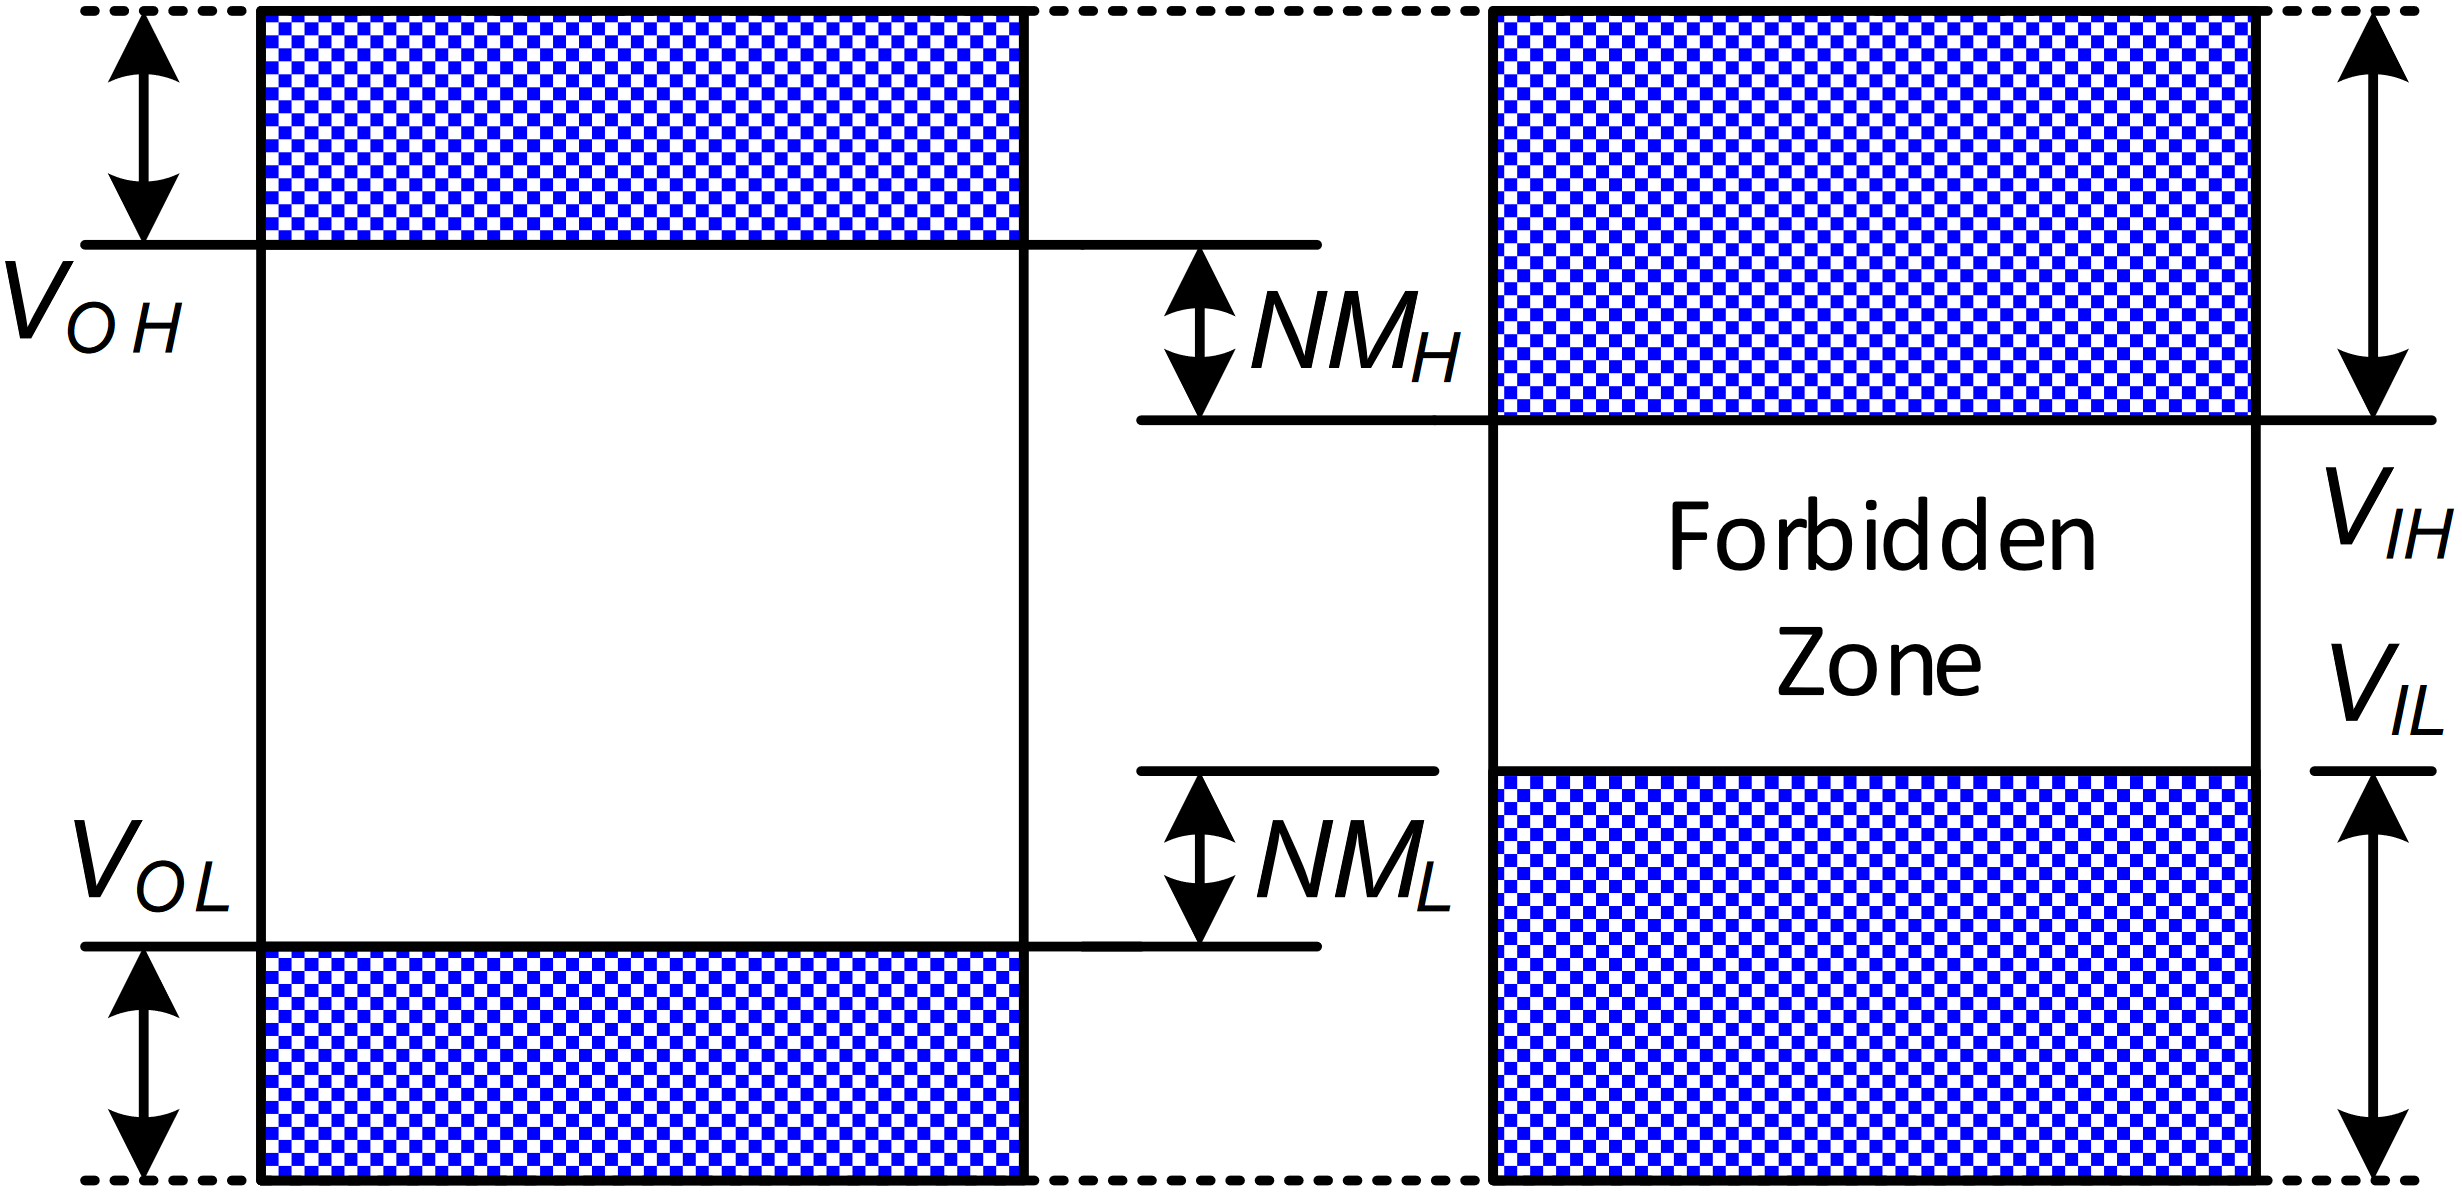
\includegraphics[width=0.30\textwidth]{MargeBruit.png}
        \end{center}
    \end{figure}

    \paragraph{Transistors}
    \mbox{}\vspace{1em}\\
    Éléments de base des circuits électroniques. Ils sont composés de 
    trois broches; le drain, la source, et la \textbf{grille} qui contrôle 
    les deux autres comme un interrupteur.  La figure suivante représente 
    un transistor hors tension \textit{off}, un transistor hors tension 
    mais polarisé \textit{off} et un transistor sous tension \textit{on}.     
    \begin{center}
    \begin{circuitikz}[scale=0.5]
    % Draw NMOS transistor
    \draw (0,0) node[nigfete] (mos) {}
    (mos.gate) node[left] {g}
    (mos.drain) node[above] {d}
    (mos.source) node[below] {s};

    % Draw NMOS in OFF state
    \draw (3,0) node[nigfete] (mosoff) {}
    (mosoff.gate) node[left] {g}
    (mosoff.drain) node[above] {d}
    (mosoff.source) node[below] {s};
    \draw (mosoff.gate) -- ++(0.5,0) node[circ] {} -- (mosoff.source);

    Draw NMOS in ON state
    \draw (6,0) node[nigfete] (moson) {}
    (moson.gate) node[left] {g}
    (moson.drain) node[above] {d}
    (moson.source) node[below] {s};
    \draw (moson.gate) -- ++(0.5,0) node[circ] {} -- (moson.drain);
    \end{circuitikz}
    \end{center}

    \paragraph{Composition d'un circuit} 
    \mbox{}\\ 
    \textbf{Circuit}$\Coloneqq$ E., S., spec. \textit{fonct}., spec. \textit{temp}.   

    \paragraph{Propriétés d'un circ. combinatoire}
    \mbox{} 
    \vspace{0.1em}
    \begin{itemize}
        \item[$\rhd$]  \textbf{Noeud} $\implies$ \textit{In}  
            ou \textbf{connexion à} un \textit{Out}. 
        \item[$\rhd$] \textbf{Aucun} chemin cyclique.    

    \end{itemize}


    \paragraph{Sommes de produits SOP}
    En considérant les variables \textit{In} d'une ligne de la table de vérité, 
    il faut identifier la \textbf{conjonction} (produit) nécessaire 
    pour engendrer un \textbf{1} logique. Un \textbf{minterm} est une 
    représentation du produit engendrant un 1 logique. 

                \begin{table}[H]
                  \begin{center}
                   \renewcommand{\arraystretch}{1.5}
                    \footnotesize
                        \begin{tabular}{|l|l|l||c|}
                        \arrayrulecolor{blue}\hline
                        \rowcolor{lightBlue}
                        \textcolor{myb}{$A$} & \textcolor{myb}{$B$} 
                                           & \textcolor{myb}{$Y$} 
                                           & \textcolor{myb}{\textit{minterm}}  
                        \\
                        \hline
                        \hline
                        \arrayrulecolor{black}
                        $V$ & $F$ & \cellcolor{myr} $0$ & $\overline{AA}$
                        \\
                        \hline
                        $0$ & $1$ & \cellcolor{myg} $1$ & \textcolor{myg}{$\overline{A}B$}
                        \\
                        \hline 
                        $1$ & $0$ & \cellcolor{myr} $0$ & $A\overline{B}$ 
                        \\ 
                        \hline
                        $1$ & $1$ & \cellcolor{myg} $1$ & \textcolor{myg}{$AB$}
                        \\
                        \hline
                        \end{tabular}
                \end{center}
                \end{table}
                \[Y(A, B) = \overline{A}B + AB \leftrightarrow Y(A,B) = \sum (1, 3) \]
    

    \paragraph{Produits de sommes}
    En considérant les variables \textit{In} d'une ligne de la table de vérité, 
    il faut identifier la \textbf{somme} nécessaire 
    pour engendrer un \textbf{0} logique. Un \textbf{maxterm} est une 
    représentation de la somme engendrant un 0 logique. 


                \begin{table}[H]
                  \begin{center}
                   \renewcommand{\arraystretch}{1.5}
                     \footnotesize
                        \begin{tabular}{|l|l|l||c|}
                        \arrayrulecolor{blue}\hline
                        \rowcolor{lightBlue}
                        \textcolor{myb}{$A$} & \textcolor{myb}{$B$} 
                                           & \textcolor{myb}{$Y$} 
                                           & \textcolor{myb}{\textit{maxterm}}  
                        \\
                        \hline
                        \hline
                        \arrayrulecolor{black}
                        $V$ & $F$ & \cellcolor{myg} $0$ & \textcolor{myg}{$A + B$}
                        \\
                        \hline
                        $0$ & $1$ & \cellcolor{myr} $1$ & $A + \overline{B}$
                        \\
                        \hline 
                        $1$ & $0$ & \cellcolor{myg} $0$ & \textcolor{myg}{$\overline{A} + B$} 
                        \\ 
                        \hline
                        $1$ & $1$ & \cellcolor{myr} $1$ & $\overline{A} + \overline{B}$ 
                        \\
                        \hline
                        \end{tabular}
                \end{center}
                \end{table}
                \[Y(A, B) = (A+B)(A + \overline{B}) = \prod (0, 2) \]



    \begin{table}[H]
      \centering
      \renewcommand{\arraystretch}{1.5}
      \setlength{\arrayrulewidth}{0.4pt}
      \arrayrulecolor{blue}
      \scriptsize
      \begin{tabular}{|l|l|l|}
        \hline
        \rowcolor{lightBlue}
        \textcolor{myb}{Axiome} & \textcolor{myb}{Dual} & \textcolor{myb}{Nom} \\
        \hline
        \hline
        \( B = 0 \) if \( B \neq 1 \) & \( B = 1 \) if \( B \neq 0 \) & Bin. field \\
        \rowcolor{lightBlue}
        \( \overline{0} = 1 \) & \( \overline{1} = 0 \) & NOT \\
        \( 0 \cdot 0 = 0 \) & \( 1 + 1 = 1 \) & AND/OR \\
        \rowcolor{lightBlue}
        \( 1 \cdot 1 = 1 \) & \( 0 + 0 = 0 \) & AND/OR \\
        \( 0 \cdot 1 \cdot 0 = 0 \) & \( 1 + 0 = 1 + 1 \) & AND/OR \\
        \hline
        \end{tabular}
    \end{table}



    \begin{table}[H]
      \centering
      \renewcommand{\arraystretch}{1.5}
      \setlength{\arrayrulewidth}{0.4pt}
      \arrayrulecolor{blue}
      \footnotesize
      \begin{tabular}{|l|l|l|}
        \hline
        \rowcolor{lightBlue}
        \textcolor{myb}{Théorème} & \textcolor{myb}{Dual} & \textcolor{myb}{Nom} \\
        \hline
        \hline
        $B \cdot 1 = B$ & $B + 0 = B$ & Identité \\
        \rowcolor{lightBlue}
        \( B \cdot  0 = 0\) & \( B + 1 = 1 \) & Élément nul \\
        \( B \cdot B = B \) & \( B + B = B \) & Indépotence \\
        \rowcolor{lightBlue}
                            & \( \overline{\overline{B}}  = B\) & Involution \\
        \( B \cdot \overline{B} = 0 \) & \( B + \overline{B} = 1 \) & Complément \\
        \hline
        \end{tabular}
    \end{table}


    \paragraph{De Morgan}
    \mbox{}\vspace{0.5em}
    \[ \neg(A + B) = \neg A + \neg B \]
    \[ \neg(A \cdot B) = \neg A \cdot \neg B \]

    \paragraph{Exemple simple de circuit combinatoire} 
    \mbox{}\vspace{0.5em}



\tikzstyle{branch}=[fill,shape=circle,minimum size=3pt,inner sep=0pt]
\begin{tikzpicture}[label distance=1mm, scale=0.75]

    \node (x0) at (0,0) {$A$};
    \node (x1) at (1,0) {$B$};
    \node (x2) at (2,0) {$C$};

    \node[not gate US, draw, rotate=-90] at ($(x2)+(0.5,-1)$) (Not2) {};
    \node[not gate US, draw, rotate=-90] at ($(x1)+(0.5,-1)$) (Not1) {};
    \node[not gate US, draw, rotate=-90] at ($(x0)+(0.5,-1)$) (Not0) {};


    \node[and gate US, draw, logic gate inputs=nnn] at ($(x2)+(2,-2)$) (And1) {};
    \node[and gate US, draw, logic gate inputs=nnn] at ($(And1)+(0,-1)$) (And2) {};
    \node[and gate US, draw, logic gate inputs=nnn] at ($(And2)+(0,-1)$) (And3) {};

    \node[or gate US, draw, rotate=-90, logic gate inputs=nnn] at ($(And3)+(1,-1)$) (Or1) {};


    \foreach \i in {0, 1, 2}
    {
        \path (x\i) -- coordinate (punt\i) (x\i |- Not\i.input);
        \draw (punt\i) node[branch] {} -| (Not\i.input);
    }




    \draw (Not0.output |- And1.input 1) node[branch] {} -- (And1.input 1);
    \draw (Not1.output |- And1.input 2) node[branch] {} -- (And1.input 2);
    \draw (Not2.output |- And1.input 3) node[branch] {} -- (And1.input 3);

    \draw (x0 |- And2.input 1) node[branch] {} -- (And2.input 1);
    \draw (Not1.output |- And2.input 2) node[branch] {} -- (And2.input 2);
    \draw (Not2.output |- And2.input 3) node[branch] {} -- (And2.input 3);


    \draw (x0 |- And3.input 1) node[branch] {} -- (And3.input 1);
    \draw (Not1.output |- And3.input 2) node[branch] {} -- (And3.input 2);
    \draw (x2 |- And3.input 3) node[branch] {} -- (And3.input 3);


     % Connect AND gates to OR gate
    \draw (And1.output) -| ([xshift=0.5cm]And1.output) -| (Or1.input 1);
    \draw (And2.output) -| ([xshift=0.5cm]And2.output) -| (Or1.input 2);
    \draw (And3.output) -| ([xshift=0.5cm]And3.output) -| (Or1.input 3);


    % Draw output from OR gate
    \draw (Or1.output)  node[below] {Y} ++(0, -0.5);

   % Additional branches for inputs
    \draw (x0) |- (And2.input 1);
    \draw (x0) |- (And3.input 1);

    \draw (Not0) |- (And1.input 1);
    \draw (Not1) |- (And1.input 2);
    \draw (Not2.output) |- (And1.input 3);


    \draw (Not1) |- (And2.input 2);
    \draw (Not2.output) |- (And2.input 3);


    \draw (x2) |- (And3.input 3);
    \draw (Not1) |- (And3.input 2);


    % Additional code to create a named coordinate at the branch point
    \path (x1) -- coordinate (branchB) (x1 |- Not1.input);

    % Now draw the line from B to the existing branch point
    \draw (x1) -- (branchB);

    \draw (And1.output) -- ++(1,0) node[right] (minterm1) {$\overline{A}\cdot\overline{B}\cdot\overline{C}$};
    \draw (And2.output) -- ++(1,0) node[right] (minterm2) {$A\overline{B}C$};
    \draw (And3.output) -- ++(1,0) node[right] (minterm3) {$AB\overline{C}$};
\end{tikzpicture}

    
    \[ Y = \overline{A}\cdot\overline{B}\cdot\overline{C} 
     + A\overline{B}\overline{C} + A\overline{B}C \]

     \paragraph{Simple règles de schématisation}
     Les \textbf{E}. sont en haut à gauche et les \textbf{S}. sont en bas à droite; 
     on utilise des \textbf{fils droits}, préférablement.   
    \vspace{1em}

\begin{center}
 \begin{tikzpicture}[node distance=1.5cm, scale=0.60]

    % Wire junction at a T
    \draw (0,0) -- (2,0);
    \draw (1,0) -- (1,-0.5);
    \node[below] at (1,-1) {(a) {Fils engendrant une jonction T}};

    % Wires connect at a dot
    \draw (0,-2) -- ++(2,0);
    \draw (1,-2) -- ++(0,-1);
    \filldraw (1,-2) circle (2pt);
    \node[below] at (1,-3) {(b) Connexion explicitée par un point};

    % Wires crossing without connecting
    \draw (0,-4) -- ++(2,0);
    \draw (1,-3.5) -- (1,-4.5);
    \node[below] at (0.75,-5) {(c) Fils croisés sans point (\;$\therefore$ non connectés)};

\end{tikzpicture}    
\end{center}

    \paragraph{Circuit de priorité}
    \mbox{}\vspace{0.5em}



\begin{center}
 \begin{tikzpicture}[scale=0.55]
    % Draw the box for the priority circuit
    \draw (0,0) rectangle (4,5);
    \node at (2,2.5) {\textit{Priorité}};

    % Draw the input lines and labels
    \draw (-1,4.5) -- (0,4.5) node[midway, above] {\(A_3\)};
    \draw (-1,3.5) -- (0,3.5) node[midway, above] {\(A_2\)};
    \draw (-1,2.5) -- (0,2.5) node[midway, above] {\(A_1\)};
    \draw (-1,1.5) -- (0,1.5) node[midway, above] {\(A_0\)};

    % Draw the output lines and labels
    \draw (4,4.5) -- (5,4.5) node[midway, above] {\(Y_3\)};
    \draw (4,3.5) -- (5,3.5) node[midway, above] {\(Y_2\)};
    \draw (4,2.5) -- (5,2.5) node[midway, above] {\(Y_1\)};
    \draw (4,1.5) -- (5,1.5) node[midway, above] {\(Y_0\)};
\end{tikzpicture}    
\end{center}


\begin{table}[H]
  \centering
  \renewcommand{\arraystretch}{1.5}
  \setlength{\arrayrulewidth}{0.4pt}
  \arrayrulecolor{blue}
  \scriptsize
  \begin{tabular}{|c|c|c|c||c|c|c|c|}
    \hline
    \rowcolor{lightBlue}
    \textcolor{myb}{$A_3$} & \textcolor{myb}{$A_2$} & \textcolor{myb}{$A_1$} & \textcolor{myb}{$A_0$} & \textcolor{myb}{$Y_3$} & \textcolor{myb}{$Y_2$} & \textcolor{myb}{$Y_1$} & \textcolor{myb}{$Y_0$} \\
    \hline
    \hline
    0 & 0 & 0 & 0 & 0 & 0 & 0 & 0 \\
    \rowcolor{lightBlue}
    0 & 0 & 0 & 1 & 0 & 0 & 0 & \textcolor{blue}{1} \\
    0 & 0 & 1 & 0 & 0 & 0 & \textcolor{blue}{1} & 0 \\
    \rowcolor{lightBlue}
    0 & 0 & 1 & 1 & 0 & 0 & \textcolor{blue}{1} & 0 \\
    0 & 1 & 0 & 0 & 0 & \textcolor{blue}{1} & 0 & 0 \\
    \rowcolor{lightBlue}
    0 & 1 & 0 & 1 & 0 & \textcolor{blue}{1} & 0 & 0 \\
    0 & 1 & 1 & 0 & 0 & \textcolor{blue}{1} & 0 & 0 \\
    \rowcolor{lightBlue}
    0 & 1 & 1 & 1 & 0 & \textcolor{blue}{1} & 0 & 0 \\
    1 & 0 & 0 & 0 & \textcolor{blue}{1} & 0 & 0 & 0 \\
    \rowcolor{lightBlue}
    1 & 0 & 0 & 1 & \textcolor{blue}{1} & 0 & 0 & 0 \\
    1 & 0 & 1 & 0 & \textcolor{blue}{1} & 0 & 0 & 0 \\
    \rowcolor{lightBlue}
    1 & 0 & 1 & 1 & \textcolor{blue}{1} & 0 & 0 & 0 \\
    1 & 1 & 0 & 0 & \textcolor{blue}{1} & 0 & 0 & 0 \\
    \rowcolor{lightBlue}
    1 & 1 & 0 & 1 & \textcolor{blue}{1} & 0 & 0 & 0 \\
    1 & 1 & 1 & 0 & \textcolor{blue}{1} & 0 & 0 & 0 \\
    \rowcolor{lightBlue}
    1 & 1 & 1 & 1 & \textcolor{blue}{1} & 0 & 0 & 0 \\
    \hline
  \end{tabular}
\end{table}

    \paragraph{Représentation d'un circuit de priorité}
    \mbox{}\vspace{0.5em}

\begin{tikzpicture}[label distance=1mm, scale=0.75]

    \node (x0) at (0,0) {$A_3$};
    \node (x1) at (1,0) {$A_2$};
    \node (x2) at (2,0) {$A_1$};
    \node (x3) at (3,0) {$A_0$};



    \node at ($(x3)+(2,-2)$) (And1) {$Y_3$};
    \node[and gate US, draw, logic gate inputs=nn] at ($(And1)+(0,-1)$) (And2) {};
    \node[and gate US, draw, logic gate inputs=nnn] at ($(And2)+(0.15,-1)$) (And3) {};
    \node[and gate US, draw, logic gate inputs=nnnn] at ($(And3)+(0.15,-1.25)$) (And4) {};


    \draw (x0) |- (And1);
    \draw (x0) |- (And1);
    \draw (And2.input 1) circle (2.5pt);
    
    \draw (x0) |-  ($(And2.input 1)+(-0.1,0)$);
    \draw (x1) |-  (And2.input 2);


    \draw (x0) |-  ($(And3.input 1)+(-0.1,0)$);
    \draw (x1) |-  ($(And3.input 2)+(-0.1,0)$);
    \draw (x2) |-  (And3.input 3);
    \draw (And3.input 1) circle (2.5pt);
    \draw (And3.input 2) circle (2.5pt);


    \draw (x0) |-  ($(And4.input 1)+(-0.1,0)$);
    \draw (x1) |-  ($(And4.input 2)+(-0.1,0)$); 
    \draw (x2) |-  ($(And4.input 3)+(-0.1,0)$);
    \draw (x3) |-  (And4.input 4);
    \draw (And4.input 1) circle (2.5pt);
    \draw (And4.input 2) circle (2.5pt);
    \draw (And4.input 3) circle (2.5pt);

    \draw ($(And2.output) + (0.5,0)$)  node[right] {$Y_2$}; 
    \draw ($(And3.output) + (0.25,0)$) node[right]{$Y_1$};
    \draw (And4.output)  node[right] {$Y_0$};

\end{tikzpicture}


\paragraph{Entrée don't care ou $\mathbb{X}$}
    Ces entrés sont utilisées pour spécifier que la variables possédant le 
    \textit{don't care} n'affecte pas le résultat de la fonction logique.   
    Une file de priorité peut être résumée par la table suivante. 


\begin{table}[H]
  \centering
  \renewcommand{\arraystretch}{1.5}
  \setlength{\arrayrulewidth}{0.4pt}
  \arrayrulecolor{blue}
  \scriptsize
  \begin{tabular}{|c|c|c|c||c|c|c|c|}
    \hline
    \rowcolor{lightBlue}
    \textcolor{myb}{$A_3$} & \textcolor{myb}{$A_2$} & \textcolor{myb}{$A_1$} & \textcolor{myb}{$A_0$} & \textcolor{myb}{$Y_3$} & \textcolor{myb}{$Y_2$} & \textcolor{myb}{$Y_1$} & \textcolor{myb}{$Y_0$} \\
    \hline
    \hline
    0 & 0 & 0 & 0 & 0 & 0 & 0 & 0 \\
    \rowcolor{lightBlue}
    0 & 0 & 0 & 1 & 0 & 0 & 0 & \textcolor{blue}{1} \\
    \rowcolor{lightBlue}
    0 & 0 & 1 & \textcolor{red}{\textit{d}}   & 0 & 0 & \textcolor{blue}{1} & 0 \\
    0 & 1 & \textcolor{red}{\textit{d}} & \textcolor{red}{\textit{d}} & 0 & \textcolor{blue}{1} & 0 & 0 \\
    \rowcolor{lightBlue}
    1 & \textcolor{red}{\textit{d}} & \textcolor{red}{\textit{d}} & \textcolor{red}{\textit{d}} & \textcolor{blue}{1} & 0 & 0 & 0 \\
    \hline
  \end{tabular}
\end{table}


    \paragraph{Contention : signal X }
    Se produit lorsque les portes logiques et les entrées sont telles 
    que la sortie à générer est \textbf{contradictoire}.   


    \begin{center}
        \begin{circuitikz}[label distance=1mm, scale=0.75]
            % Define the NOT gates
            \node[not port] (not1) at (0,0) {};
            \node[not port] (not2) at (0,-2) {};
            \node (jonction) at (1,-1) {};

            % Connect the NOT gates outputs to the same node (contention)
            \draw (not1.out) -| (1,-1) node[above right] {$Y=\mathbb{X}$};    
            \draw (not2.out) -| (1,-1);
            % Connect the NOT gates inputs to the labels
            \draw (not1.in) -- ++(-1,0) node[left] {$A = 1$};
            \draw (not2.in) -- ++(-1,0) node[left] {$B = 0$};
        \end{circuitikz}        
    \end{center}



    \paragraph{Tampon à trois états : signal $\mathbb{Z}$}
    Circuit dans lequel une entrée $\mathbb{E}$ est connecté à une porte tampon et contrôle 
    la \textbf{propagation du signal}. Lorsque l'entrée $\mathbb{E}$ est 
    sous tension haute, la porte agit comme un tampon normal; lorsque l'entrée 
    $\mathbb{E}$ est sous tension basse, la porte produit le signal $\mathbb{Z}$ qui 
    indique que $A$ est \textit{contrôlé}.   

    \begin{center}
        \begin{circuitikz}[scale=0.5]
        % Define buffer gate
        \node[buffer] (buf) at (0,0) {};
        
        % Draw input and output lines
        \draw (buf.in) -- ++(-1,0) node[left] {$A$};
        \draw (buf.out) -- ++(1,0) node[right] {$Y$};
        
        % Draw enable line
        \draw ($(buf.in) + (1, 1)$) -- ++(0,1) node[above] {$E$};
        \end{circuitikz}        
    \end{center}


    \paragraph{Méthodes de Karnaugh}
    Méthode \textbf{graphique}   
    permettant de simplifier les formules de circuits 

    \begin{itemize}
        \item[$\rhd$]   \textbf{Organiser}  les éléments en grille 
            de façon à ce que chaque cellule ne diffère d'une 
            cellule voisine que par \textbf{1 bit}.   
        \item[$\rhd$] Remplir la grille de façon à refléter le 
            \textbf{tableau d'origine}.   
        \item[$\rhd$] \textbf{Grouper} ou entourer les cellules 
            adjacentes qui possèdent un \textbf{1}.   
    \end{itemize}   


    \begin{table}[H]
    \centering
    \footnotesize
    \begin{tabular}{|c|c|c||c|}
    \hline
    \rowcolor{lightBlue}
    \textcolor{myb}{$A$} & \textcolor{myb}{$B$} 
                       & \textcolor{myb}{$C$} 
                       & \textcolor{myb}{$Y$}\\
    \hline
    \hline
    0 & 0 & 0 & \textcolor{blue}{1}   \\ 
    \rowcolor{lightBlue}
    0 & 0 & 1 & \textcolor{blue}{1} \\ 
    \rowcolor{lightBlue}
    0 & 1 & 0 & 0 \\
    0 & 1 & 1 & 0 \\
    \rowcolor{lightBlue}
    1 & 0 & 0 & 0 \\
    1 & 0 & 1 & 0 \\
    \rowcolor{lightBlue}
    1 & 1 & 0 & 0 \\
    1 & 1 & 1 & 0 \\
    \hline
  \end{tabular}
\end{table}        


    \begin{center}
        \begin{karnaugh-map}[4][2][1][$B$][$A$][$C$][$$]
            \minterms{0,4}
            \autoterms[0] 
            \implicant{0}{4}
        \end{karnaugh-map}
    \end{center}


    \begin{center}
        \begin{karnaugh-map}[4][2][1][$B$][$A$][$C$][$$]
          \terms{0}{\tiny{$\overline{A}\cdot\overline{B}\cdot\overline{C}$}}
            \terms{4}{\tiny{$\overline{A}\cdot\overline{B}C$}}
            \autoterms[0]
        \end{karnaugh-map}
    \end{center}
    \textbf{Solution} : considérer les variables qui ne changent pas 
    leurs valeurs entre les cases \textbf{groupés}. Ici, la variable 
    $C$ change de valeur entre le cellule 1 et la cellule 2; 
    elle n'est donc pas considérée dans \textbf{l'équation simplifiée}. 
    Nous avons alors :
    \[Y = \overline{A}\overline{B} \]

    \paragraph{Autre exemple de Karnaugh-map de 3 entrées}
    Parfois, il y a plusieurs \textbf{implicants}. 
    \begin{table}[H]
    \centering
    \footnotesize
    \begin{tabular}{|c|c|c||c|}
    \hline
    \rowcolor{lightBlue}
    \textcolor{myb}{$A$} & \textcolor{myb}{$B$} 
                       & \textcolor{myb}{$C$} 
                       & \textcolor{myb}{$Y$}\\
    \hline
    \hline
    0 & 0 & 0 & 0 \\ 
    \rowcolor{lightBlue}
    0 & 0 & 1 & 0 \\ 
    \rowcolor{lightBlue}
    0 & 1 & 0 & \textcolor{blue}{1} \\
    0 & 1 & 1 & \textcolor{blue}{1} \\
    \rowcolor{lightBlue}
    1 & 0 & 0 & 0 \\
    1 & 0 & 1 & 0 \\
    \rowcolor{lightBlue}
    1 & 1 & 0 & \textcolor{blue}{1} \\
    1 & 1 & 1 & 0 \\
    \hline
  \end{tabular}
\end{table}        


    \begin{center}
      \tiny
        \begin{karnaugh-map}[4][2][1][$B$][$A$][$C$][$$]
            \minterms{1,3,5}
            \autoterms[0] 
            \implicant{1}{3}
            \implicant{1}{5}
        \end{karnaugh-map}
    \end{center}
    \[ Y = \overline{A}B + B\overline{C} \] 


     \paragraph{Autre exemple de Karnaugh-map de 3 entrées}
     Pour les tables de Karnaugh à 4 entrées et plus, les implicants 
     devinnent plus complexes. 

  \begin{table}[H]
    \centering
    \renewcommand{\arraystretch}{1.15}
    \setlength{\arrayrulewidth}{0.4pt}
    \arrayrulecolor{blue}
    \scriptsize
    \begin{tabular}{|c|c|c|c||c|}
      \hline
      \rowcolor{lightBlue}
      \textcolor{myb}{$A$} & \textcolor{myb}{$B$} & \textcolor{myb}{$C$} & \textcolor{myb}{$D$} & \textcolor{myb}{$Y$} 
      \\ \hline
      0 & 0 & 0 & 0 & \textcolor{blue}{1} \\
      \rowcolor{lightBlue}
      0 & 0 & 0 & 1 & 0 \\
      0 & 0 & 1 & 0 &  \textcolor{blue}{1}  \\
      \rowcolor{lightBlue}
      0 & 0 & 1 & 1 & \textcolor{blue}{1} \\
      0 & 1 & 0 & 0 & 0 \\
      \rowcolor{lightBlue}
      0 & 1 & 0 & 1 & \textcolor{blue}{1}  \\
      0 & 1 & 1 & 0 & \textcolor{blue}{1}  \\
      \rowcolor{lightBlue}
      0 & 1 & 1 & 1 & \textcolor{blue}{1} \\
      1 & 0 & 0 & 0 & \textcolor{blue}{1} \\
      \rowcolor{lightBlue}
      1 & 0 & 0 & 1 & \textcolor{blue}{1} \\
      1 & 0 & 1 & 0 & \textcolor{blue}{1} \\
      \rowcolor{lightBlue}
      1 & 0 & 1 & 1 & 0 \\
      1 & 1 & 0 & 0 & 0 \\
      \rowcolor{lightBlue}
      1 & 1 & 0 & 1 & 0 \\
      1 & 1 & 1 & 0 & 0 \\
      \rowcolor{lightBlue}
      1 & 1 & 1 & 1 & 0 \\
      \hline
    \end{tabular}
  \end{table}


  \begin{center}
      \tiny
        \begin{karnaugh-map}[4][4][1][$B$][$A$][$D$][$C$]
            \minterms{0, 2, 5, 6, 12, 13, 8, 9, 10}
            \implicant{2}{6}
            \implicantcorner
            \implicant{12}{9}
            \implicant{5}{13}
        \end{karnaugh-map}
  \end{center}


  \paragraph{Karnaugh-map avec Don't Cares}
  Les \textit{don't care} peuvent complexifier la simplifiation de la 
  fontion à cause du plus grand nombre de \textbf{cas possibles}
  lors du regroupement. 



  \begin{table}[H]
    \centering
    \renewcommand{\arraystretch}{1.5}
    \setlength{\arrayrulewidth}{0.4pt}
    \arrayrulecolor{blue}
    \scriptsize
    \begin{tabular}{|c|c|c|c||c|}
      \hline
      \rowcolor{lightBlue}
      \textcolor{myb}{$A$} & \textcolor{myb}{$B$} & \textcolor{myb}{$C$} & \textcolor{myb}{$D$} & \textcolor{myb}{$Y$} 
      \\ \hline
      0 & 0 & 0 & 0 & \textcolor{blue}{1} \\
      \rowcolor{lightBlue}
      0 & 0 & 0 & 1 & 0 \\
      0 & 0 & 1 & 0 &  \textcolor{blue}{1}  \\
      \rowcolor{lightBlue}
      0 & 0 & 1 & 1 & \textcolor{blue}{1} \\
      0 & 1 & 0 & 0 & 0 \\
      \rowcolor{lightBlue}
      0 & 1 & 0 & 1 & \textcolor{red}{$\mathbb{X}$}    \\
      0 & 1 & 1 & 0 & \textcolor{blue}{1}  \\
      \rowcolor{lightBlue}
      0 & 1 & 1 & 1 & \textcolor{blue}{1} \\
      1 & 0 & 0 & 0 & \textcolor{blue}{1} \\
      \rowcolor{lightBlue}
      1 & 0 & 0 & 1 & \textcolor{blue}{1} \\
      1 & 0 & 1 & 0 & \textcolor{blue}{1} \\
      \rowcolor{lightBlue}
      1 & 0 & 1 & 1 & \textcolor{red}{$\mathbb{X}$} \\
      1 & 1 & 0 & 0 & \textcolor{red}{$\mathbb{X}$} \\
      \rowcolor{lightBlue}
      1 & 1 & 0 & 1 & \textcolor{red}{$\mathbb{X}$} \\
      1 & 1 & 1 & 0 & \textcolor{red}{$\mathbb{X}$} \\
      \rowcolor{lightBlue}
      1 & 1 & 1 & 1 & \textcolor{red}{$\mathbb{X}$} \\
      \hline
    \end{tabular}
  \end{table}

  


  
  % paragraph  (end)


  \begin{center}
      \tiny
        \begin{karnaugh-map}[4][4][1][$B$][$A$][$D$][$C$]
            \minterms{0,2,6, 12, 13, 8,9}
            \terms{3,5,7, 15, 14, 13, 10}{$\mathbb{X}$}
            \implicantcorner
            \implicant{3}{10}
            \implicant{12}{10}
        \end{karnaugh-map}
  \end{center}

  \[ Y = A + \overline{B} \cdot \overline{D} + C \]


  \paragraph{Karnaugh-map de 5 entrées}
  Il faut considérer \textbf{deux} K-map de \textbf{quatre} variables. Par convention, 
  on peut omettre la première variable dans les deux K-map; on considère que la 
  dans la première K-map, la variable irgnorée a une valeur de \textbf{0} et, dans la 2e K-map, 
  elle a une valeur de \textbf{1}. 
  \href{https://www.youtube.com/watch?v=CZPwYZdmMI0&t=417s}{\texttt{Exemple sur Youtube}} 
  Soit la fonction et K-maps correspondantes :  
  \begin{align*}
    f(A, B, C, D, E) = &\sum(0, 1, 2, 4, 5, 6, 10, 13, 
                    \\ &14 18, 21, 22, 24, 26, 29, 30)
  \end{align*}


  \begin{figure}[H]  
    \caption*{\footnotesize{K-map de $BCDE$ en considérant $A = 0$}}
    \begin{center}
        \begin{karnaugh-map}[4][4][1][$C$][$B$][$E$][$D$]
          \terms{0}{1\;\tiny{\textcolor{myp}{0}}}
          \terms{1}{1\;\tiny{\textcolor{myp}{1}}}
          \terms{4}{1\;\tiny{\textcolor{myp}{4}}}
          \terms{5}{1\;\tiny{\textcolor{myp}{5}}}
          \terms{7}{1\;\tiny{\textcolor{myp}{7}}}
          \terms{8}{1\;\tiny{\textcolor{myp}{8}}}
          \terms{9}{1\;\tiny{\textcolor{myp}{9}}}
          \terms{10}{1\;\tiny{\textcolor{myp}{10}}}
          \terms{11}{1\;\tiny{\textcolor{myp}{11}}}
          \terms{2}{0\;\tiny{\textcolor{myp}{2}}}
          \terms{3}{0\;\tiny{\textcolor{myp}{3}}}
          \terms{6}{0\;\tiny{\textcolor{myp}{6}}}
          \terms{12}{0\;\tiny{\textcolor{myp}{12}}}
          \terms{13}{0\;\tiny{\textcolor{myp}{13}}}
          \terms{14}{0\;\tiny{\textcolor{myp}{14}}}
          \terms{15}{0\;\tiny{\textcolor{myp}{15}}}
            \minterms{0, 1, 4, 5, 7, 8, 9, 11, 10}
            \implicant{0}{5}
            \implicant{5}{7}
            \implicant{8}{10}
        \end{karnaugh-map}    \end{center}
  \end{figure}

  \[ \textcolor{myyellow!50}{D\overline{E}} + \textcolor{green}{C\overline{D} \cdot E}   
  + \textcolor{red}{\overline{A} \cdot \overline{B} \cdot \overline{D}}  \]
    


   \begin{figure}[H]
    \caption*{\footnotesize{K-map de $BCDE$ en considérant $A = 1$}}
    \begin{center}
    
      \begin{karnaugh-map}[4][4][1][$C$][$B$][$E$][$D$]
          \terms{0}{0\;\tiny{\textcolor{myp}{16}}}

          \terms{1}{0\;\tiny{\textcolor{myp}{17}}}
          
          \terms{4}{0\;\tiny{\textcolor{myp}{20}}}
          \terms{5}{1\;\tiny{\textcolor{myp}{21}}}
          \terms{7}{1\;\tiny{\textcolor{myp}{23}}}


          \terms{8}{1\;\tiny{\textcolor{myp}{24}}}
          \terms{9}{1\;\tiny{\textcolor{myp}{25}}}
          \terms{10}{1\;\tiny{\textcolor{myp}{26}}}
          \terms{11}{1\;\tiny{\textcolor{myp}{27}}}
          \terms{2}{0\;\tiny{\textcolor{myp}{18}}}
          \terms{3}{0\;\tiny{\textcolor{myp}{19}}}
          \terms{6}{0\;\tiny{\textcolor{myp}{22}}}

          \terms{12}{0\;\tiny{\textcolor{myp}{28}}}
          \terms{13}{0\;\tiny{\textcolor{myp}{29}}}
          \terms{14}{0\;\tiny{\textcolor{myp}{28}}}
          \terms{15}{0\;\tiny{\textcolor{myp}{31}}}
            \minterms{2, 5, 7, 8, 9, 10, 11}
            \implicantedge{2}{2}{10}{10}
            \implicant{5}{7}
            \implicant{8}{10}
        \end{karnaugh-map}    \end{center}
    \caption{}
  \end{figure}


  \[ \textcolor{myyellow!50}{D\overline{E}} + \textcolor{green}{C\overline{D} \cdot E}   
  + \textcolor{red}{A B \cdot \overline{C}}  \]

  \paragraph{Karnaugh-map de 6 entrées}
  \mbox{}\vspace{0.5em}
  \begin{note}{}{}
        On peut utiliser la même approches que la méthode pour entrée, cette fois 
        en considérant \textbf{4} K-map de 4 variables superposées dans un cube 
        tridimensionnel
        \href{https://www.youtube.com/watch?v=LXJXZOqZpGk}{Exemple sur \texttt{Youtube}}
  \end{note}
    \paragraph{Multiplexeur}
    \begin{itemize}
        \item[$\rhd$]  $2^n$ lignes d'entrées 
        \item[$\rhd$]  $2^n$ N lignes de sélections 
        \item[$\rhd$]  $2^n$ Une seule sorties $Y$  
    \end{itemize}
    Possède deux implémentations secondaires, soit (1) \textbf{portes logiques}
    et (2) \textbf{tampons} à trois états. 
    \end{multicols*}

\end{document}
